\chapter{Prestations sociales}
\section{Introduction et objectifs}
\subsection{Introduction}
Dans ce chapitre, nous discutons de plusieurs prestations sociales que les contribuables peuvent recevoir et de la manière dont ils sont traités comme un revenu dans les déclarations de revenus. Nous discutons également des prestations reçues du Régime de rentes du Québec, de l'assurance-emploi fédérale et de l'assurance parentale du Québec. Certaines prestations peuvent devoir être remboursées et nous discutons du traitement fiscal de ces remboursements. Enfin, nous étudions le traitement fiscal des frais juridiques , des dons de bienfaisance et de deux principaux crédits d'impôt remboursables disponibles pour les revenus d'emploi faibles à modestes.


\subsection{Objectifs}
\begin{itemize}[label=\twemoji{check mark button}]
	\item Expliquer le Programme de protection des salariés et déclarer les sommes reçues;
	\item Déclarer les indemnités pour les accidents du travail, pour les accidentés de la route et pour les victimes d'acte criminel;
	\item Déclarer les prestations d'assistance sociale, et toute aide financière semblable;
	\item Déclarer les sommes reçues du Régime de rentes du Québec;
	\item Déclarer les prestations d'assurance-emploi;
	\item Déterminer le montant du remboursement des prestations d'assurance-emploi et le traiter;
	\item Déclarer les prestations versées par le gouvernement fédéral et Québec à cause de la COVID-19;
	\item Déclarer les prestations d'assurance parentale;
	\item Déclarer les \og Autres revenus \fg{} et \og Autres montants \fg{};
	\item Identifier les frais juridiques que le contribuable peut déduire;
	\item Réclamer les \og Autres déductions \fg{};
	\item Réclamer le montant pour l'achat d'une habitation au fédéral et Québec;
	\item Identifier les dons qui sont considérés comme des dons de bienfaisance, et calculer le crédit d'impôt non remboursable relatif à ces dons;
	\item Aux fins de l'impôt du Québec, expliquer en quoi consiste le crédit pour la prime au travail, le crédit pour la prime au travail adaptée et le crédit pour le supplément à la prime au travail, et les réclamer;
	\item Aux fins de l'impôt fédéral, expliquer en quoi consiste le crédit d'impôt pour allocation canadienne pour les travailleurs, et le réclamer;
	\item Expliquer les conditions à remplir pour bénéficier de crédit d'impôt Bouclier fiscal, et le réclamer;
	\item Expliquer en quoi consiste le crédit d'impôt pour mise aux normes d'installations d'assainissement des eaux usées résidentielles offert par le gouvernement du Québec, et le réclamer.
\end{itemize}


\subsection{Sujets du chapitre}
\begin{itemize}
	\item CNESST
	\item Prestations RRQ, RQAP, et AE
	\item Achat habitation
	\item Bouclier fiscal
	\item Aide financière aux familles
	\item Dons
	\item ACT et Prime au travail
\end{itemize}



\section{T5007 et Relevé~5}
\begin{intro}
	Dans les prochaines parties, nous allons discuter de plusieurs prestations sociales qui sont inscrites sur le T5007 et le Relevé~5.
	
	Vous remarquerez que le Québec accorde des indemnités qui ne sont pas inscrites comme revenu sur le feuillet fédéral. Ces indemnités sont exonérées d'impôt sur la T1.
\end{intro}


\subsection{T5007}
Le feuillet fiscal \href{https://www.canada.ca/fr/agence-revenu/services/formulaires-publications/formulaires/t5007.html}{T5007} est émis pour enregistrer les paiements pour les prestations fédérales suivantes:
\begin{itemize}
	\item Indemnité pour accidents du travail;
	\item Prestation d'assistance sociale.
\end{itemize}


\subsection{Relevé~5}
Le \href{https://www.revenuquebec.ca/fr/services-en-ligne/formulaires-et-publications/details-courant/rl-5/}{Relevé~5} est émis pour enregistrer les versements des prestations et indemnités suivantes versées par le Québec: 
\begin{itemize}
	\item CNESST
	\item Assistance sociale
	\item Aide financière gouvernementale
	\item Indemnités de la SAAQ
	\item Indemnités pour actes de civisme, victimes d'actes criminels, arrêt préventif d'activité et aide au remplacement du revenu.
\end{itemize}



\section{Accidents du travail}
\begin{intro}
	L'indemnisation des victimes d'accident du travail est une sorte d'assurance qui vise à compenser les difficultés occasionnées par une maladie, un accident ou un décès liés au travail. Le programme, financé par des cotisations patronales basées sur la masse salariale, est utilisé pour couvrir les coûts des soins médicaux et de la réadaptation des travailleurs.
\end{intro}

\index{Travailleur}
Dans ce contexte, un \og travailleur \fg{} est une personne qui exerce un travail rémunéré pour un employeur en vertu d'un contrat de travail.

Dans les provinces et territoires du Canada, il existe des lois qui établissent les droits et les obligations des travailleurs et des employeurs lorsqu'il y a une maladie, un accident ou un décès relié au travail. Au Québec, on retrouve la \acrfull{lsst}, qui traite de la prévention et de l'inspection, et la \acrfull{latmp}, qui régit l'indemnisation et la réadaptation des travailleurs.

En général, ces lois confient aux employeurs et aux travailleurs la responsabilité de la santé et de la sécurité au travail dans leur milieu de travail. La \acrfull{cnesst} est chargée de leur application. 


\subsection{Qui verse les indemnités pour un accident du travail?}
Les indemnités pour un accident du travail sont versées par la CNESST. Cet organisme remet un feuillet~T5007 et un relevé~5 aux personnes qui ont reçu des indemnités durant l'année d'imposition.

Les prestations versées par la CNESST sont indiquées à la case~10 du feuillet~T5007 et à la case~C du Relevé~5. Ces prestations ne sont \textbf{pas imposables}; cependant, ils doivent être inclus dans le revenu total et le revenu net avant d'être déduits avant le revenu imposable.

\subsection{Attente d'une décision de la CNESST}
En attendant la décision de la CNESST, l'employeur peut continuer à verser des sommes à l'employé. Ces montants sont déclarés selon la nature du revenu:
\begin{itemize}
	\item Si l'employeur lui verse un salaire, le montant constitue un revenu d'emploi et sera déclaré sur des T4 et relevé~1;
	\item S'il lui verse une avance sur indemnités, aucun montant ne doit être déclaré parce que cette somme sera remboursée par la CNESST à l'employeur lorsque la demande sera approuvée;
	\item S'il lui verse un prêt, aucun montant ne doit être déclaré;
	\item S'il lui verse des prestations d'assurance salaire provenant d'un régime collectif d'assurance salaire, l'imposition de ce revenu dépend de la personne qui a versé les cotisations au régime et du degré de contrôle exercé par l'employeur sur le régime. Si nécessaire, revoir la discussion sur ce sujet au chapitre 2.
\end{itemize}

\subsubsection{Remboursement des sommes versées par l'employeur}
Lorsque la CNESST reconnaît que l'employé a droit à une indemnité, les sommes versées par l'employeur durant la période d'attente d'une décision de la CNESST lui sont remboursées. Elles constituent des indemnités de remplacement du revenu et l'employé recevra un feuillet~T5007 et un relevé~5. 

Il arrive que la demande soumise à la CNESST soit approuvée dans une année subséquente. Par exemple, si une demande déposée en 2022 est approuvée en 2023, l'employé peut avoir déclaré les sommes versées par l'employeur à titre de revenus imposables en 2022. En 2023, lorsque la demande est approuvée, l'employeur reçoit un remboursement de la CNESST. L'employeur émettra les feuillets suivants:

\begin{itemize}[label=\twemoji{check box with check}]
	\item Un T4 avec le montant du remboursement à la case~77:
	\begin{itemize}
		\item Le contribuable pourra réclamer une déduction correspondant au remboursement à la ligne~22900 de sa T1;
	\end{itemize}
	\item Un relevé~1 avec le montant du remboursement:
	\begin{itemize}
		\item À la case~A-3;
		\item À la case~O-4, si la somme versée par l'employeur a été déclarée à titre de prestations d'assurance salaire.
	\end{itemize}
\end{itemize}

Le contribuable pourra réclamer une déduction correspondant au remboursement à la ligne~207, avec le code \og 12 \fg{} à la case~206, de sa TP-1, que ce soit le code A-3 ou O-4 sur le relevé~1.

\subsection{Indemnité pour retrait préventif}
Le \og retrait préventif \fg{} consiste en un ensemble de mesures qui permet à un travailleur d'accomplir son travail en sécurité. Il doit être justifié par un certificat visant le retrait préventif, rempli, daté et signé par un médecin. 

Les indemnités pour retrait préventif sont inscrites aux cases~10 du T5007 et E du relevé~5. Elles doivent être incluses dans le revenu à la ligne~14400 de la T1 et à la ligne~148 de la TP-1, en utilisant le code 02 à la case~149.

\subsection{Recouvrement d'indemnités versées en trop}
Au fédéral, l'ARC ne considère pas une indemnité versée en trop comme étant une indemnité pour le contribuable qui l'a reçue. L'employeur ne doit pas inclure la somme payée en trop dans le revenu du contribuable pour l'année du paiement. En effet, si le contribuable rembourse la somme au cours de la même année ou rembourse une année suivante, il n'y a aucune déduction lui permettant de la déduire de son revenu. 

Dans ce cas, la CNESST doit émettre un T5007 modifié pour l'année où la somme a été versée en trop au contribuable, et non pour l'année où elle a découvert ou récupéré le paiement en trop. Le contribuable doit alors procéder au redressement de sa déclaration fédérale de l'année en question.

Au Québec, si le montant des indemnités remboursées dépasse le montant des indemnités reçues dans l'année, le payeur inscrit l'excédent à la case~P du relevé~5. Si les sommes remboursées ont déjà été incluses dans le revenu du contribuable de l'année courante ou dans celui d'une année antérieure, le contribuable peut réclamer une déduction à la ligne~246 de la TP-1. De plus, il doit l'ajouter à son revenu net à la ligne~276, code \og 02 \fg{} à la case~277, de la TP-1.



\section{Société de l'assurance automobile du Québec (SAAQ)}
\begin{intro}
	La Société de l'assurance automobile du Québec (SAAQ) utilise le relevé~5 pour reporter les indemnités de remplacement du revenu, qu'elle a versées au contribuable à la suite d'un accident de la route.
\end{intro}

La \acrfull{saaq} utilise le relevé~5 pour reporter les indemnités de remplacement du revenu, qu'elle a versées au contribuable à la suite d'un accident de la route.

Le contribuable doit reporter le montant de la case~D du relevé~5:
\begin{itemize}
	\item À la ligne~148, avec le code \og 03 \fg{} à la case~149, de la TP-1;
	\item Comme les indemnités reçues ne sont pas imposables, une déduction correspondante peut être réclamée à la ligne~295 de la TP-1;
	\item Il n'y a aucun feuillet~T5007 pour ces indemnités, parce que le contribuable n'a pas à les déclarer sur sa T1.
\end{itemize}


Il est possible que le contribuable ait reçu d'autres sommes de la SAAQ, mais que celles-ci ne soient pas incluses dans le montant de la case~D. Ces sommes ne doivent pas être déclarées sur la TP-1, car elles ne sont pas considérées comme des indemnités de remplacement du revenu.


\subsection{Remboursement des indemnités à la SAAQ}
Si le montant des indemnités remboursées dépasse le montant des indemnités reçues dans l'année courante, l'administrateur de la SAAQ inscrit l'excédent à la case~P du relevé~5. 

Si les sommes remboursées ont déjà été incluses dans le revenu du contribuable de l'année courante ou dans celui d'une année antérieure, il peut réclamer une déduction à la ligne~246 de la TP-1. De plus, il doit l'ajouter à son revenu net à la ligne~276, code \og 02 \fg{} à la case~277, de la TP-1.



\section{Victime d'un acte criminel}
\begin{intro}
	Un contribuable peut recevoir des indemnités de remplacement du revenu pour la perte d'un soutien financier en raison d'un acte de civisme ou à titre de victime d'un acte criminel, ou une compensation pour la perte d'un soutien financier en vertu d'une loi du Canada ou d'une province autre que la province de Québec. 
\end{intro}

Ces indemnités sont inscrites à la case~E du relevé~5. Le montant doit être reporté à la ligne~148, avec le code \og 05 \fg{} à la case~149, de la TP-1.
Toutefois, une déduction peut être réclamée correspondant au montant de la case~E, à la ligne~295 de la TP-1.

Le contribuable québécois ne devrait pas recevoir de feuillet~T5007, car ce revenu n'est déclaré qu'au Québec. 

Toutefois, s'il a reçu une indemnité de remplacement de revenu en vertu d'une loi du Canada ou d'une autre province qui ne figure pas sur un relevé~5, il ne doit pas déclarer ce type d'indemnités sur sa déclaration fédérale, mais il doit le faire sur sa déclaration~TP-1. Cependant, ces montants doivent être déclarés sur leur déclaration~TP-1 comme un revenu à la ligne~148 et la déduction correspondante réclamée à la ligne~295.


\section{Redressement pour indemnités de remplacement du revenu}
\begin{intro}
	Au Québec, le contribuable qui a reçu des indemnités de remplacement du revenu, ou une compensation pour la perte d'un soutien financier doivent réduire son montant personnel de base.
\end{intro}



Le montant du redressement est indiqué à la case~M du Relevé~5 et ce montant a été pris en compte dans le calcul des indemnités ou compensations reçues.

Les contribuables doivent inscrire le montant qui figure à la case~M du relevé~5 à la ligne~358 de leur TP-1. La ligne~358 est alors soustraite de la ligne~350, ce qui signifie que la case~M du Relevé~5 réduit le montant personnel de base.

Les indemnités qui exigent un redressement comprennent:
\begin{itemize}
	\item Les indemnités pour accident du travail;
	\item Les indemnités pour retrait préventif;
	\item Les indemnités pour la perte d'un soutien financier en raison d'un acte de civisme ou à titre de victime d'un acte criminel;
	\item Les indemnités versées par la SAAQ pour un accident de la route.
\end{itemize}

Le redressement maximal pour indemnité de remplacement du revenu prévu à la ligne~358 est de \numprint{15464,70}~\$ pour 2023, soit 90~\% du montant personnel de base.

Si un résident du Québec a reçu des indemnités de remplacement du revenu ou une compensation pour la perte d'un soutien financier, en vertu d'une loi du Canada ou d'une province autre que le Québec, il doit remplir le formulaire \href{https://www.revenuquebec.ca/fr/services-en-ligne/formulaires-et-publications/details-courant/tp-752-0-0-6/}{TP-752.0.0.6, Redressement pour indemnités de remplacement du revenu reçues d'un régime public d'indemnisation hors du Québec}, afin de déterminer le montant du redressement d'impôt qu'il doit inscrire à la ligne~358 de sa déclaration provinciale. 

Pour compléter le formulaire provincial TP-752.0.0.6, il doit obtenir les taux, les montants ou tout autre renseignement requis pour le calcul du redressement d'impôt, de l'organisme situé à l'extérieur du Québec qui lui a versé ces indemnités. 
\rqg{50}



\section{Assistance sociale}
\begin{intro}
	L'assistance sociale est une aide financière payée par le gouvernement du Québec, dans le but de fournir un revenu de subsistance au contribuable qui ne peut pas subvenir à ses besoins à cause d'un manque de travail, de maladie, de blessure, d'invalidité ou d'autres motifs.
\end{intro}


\subsection{Programmes d'aide financière de dernier recours}
La prestation d'assistance sociale est versée par le ministère du Travail, de l'Emploi et de la Solidarité sociale (MTESS). Elle n'est \textbf{pas imposable au fédéral}, mais elle est \textbf{imposable au Québec}.

\begin{itemize}
	\item Le \og programme d'aide sociale \fg{} qui s'adresse aux individus sans contraintes sévères à l'emploi, et le \og programme de solidarité sociale \fg{} qui vise ceux présentant des contraintes sévères à l'emploi. Les montants versés dans le cadre de ces programmes figurent aux cases~11 du T5007 et A du relevé~5;
	\item Le \og Programme objectif emploi \fg{} vise à offrir un accompagnement personnalisé aux personnes qui auraient droit de bénéficier, pour une 1ère fois, d'une prestation du Programme d'aide sociale, pour que ces derniers puissent intégrer le marché du travail et acquérir une autonomie financière. L'aide financière reçue est indiquée aux cases~11 du T5007 et B du relevé~5.
\end{itemize}

Sur la déclaration T1, une déduction correspondante peut être réclamée à la ligne~25000.


\subsection{Prestations d'assistance sociale réclamées par un couple qui vivait ensemble}
Au fédéral, lorsque les prestations ont été reçues par un couple qui vivait ensemble au moment où les prestations sont versées, c'est le conjoint ayant le revenu net le plus élevé qui doit les déclarer à la ligne~14500 de la T1. Par la suite, elles peuvent être déduites à la ligne~25000 de la déclaration T1 du conjoint qui les a déclarées. Si les deux conjoints ont un revenu net similaire, c'est la personne dont le nom figure sur le feuillet~T5007 qui doit les déclarer.

Au Québec, chaque conjoint reçoit un relevé~5 et doit déclarer les prestations reçues à la ligne~147 de leur TP-1 respective. Il n'y a aucune déduction au Québec, car les montants versés sont imposables. 


\subsection{Remboursement de prestations d'assistance sociale reçues en trop}
L'ARC ne considère pas des prestations d'assistance sociale payées en trop comme des prestations pour le contribuable qui les a reçues. Elles ne doivent pas être incluses dans le revenu du contribuable pour l'année du remboursement. En effet, si le contribuable rembourse la somme au cours de la même année ou la rembourse l'année suivante, il n'y a aucune déduction qui peut lui permettre de déduire la somme payée en trop de son revenu.

Par ailleurs, un feuillet~T5007 modifié doit être émis pour l'année où le paiement en trop a été versé au contribuable, et non pour l'année où le paiement en trop a été découvert ou récupéré. Le contribuable doit alors rajuster sa déclaration fédérale de l'année en question. 

Au Québec, les montants remboursés dans l'année sont indiqués à la case~H du relevé~5. Ce montant est déductible à la ligne~246 de la TP-1. 

\cat\href{https://www.canada.ca/fr/agence-revenu/services/formulaires-publications/trousses-impot-toutes-annees-imposition/trousse-generale-impot-prestations/5000-g.html}{Renseignements sur l'impôt fédéral et les prestations pour 2023}

\rqg[s]{28 et 39}



\section{Programme de protection des salariés}
\begin{intro}
	Le \acrfull{pps} est un programme créé par le gouvernement du Canada. Il a pour but de protéger le salaire et les vacances impayés de tout employé admissible en cas de faillite ou de mise sous séquestre de son employeur. Les sommes versées par ce programme sont imposables.
\end{intro}

Le contribuable peut soumettre sa demande dans le cadre du PPS en remplissant le \href{https://srv217.services.gc.ca/ihst4/Intro.aspx?cid=08874c44-77de-42ca-8a48-d933ddbd3de3&lc=fra}{Formulaire de demande dans le cadre du programme de protection des salariés}, qu'il peut se procurer auprès de Service Canada. La demande doit être soumise dans les 56 jours suivant la date de la déclaration de la faillite ou de la mise sous séquestre.

Le contribuable peut soumettre une demande de prestations du PPS s'il remplit les conditions suivantes:
\begin{itemize}
	\item Son emploi a pris fin;
	\item Son employeur a déclaré faillite ou a été mis sous séquestre;
	\item Son ancien employeur lui doit un salaire admissible gagné pendant la période de six mois précédant la date de la faillite ou de la mise sous séquestre;
	\item La faillite ou la mise sous séquestre de son ancien employeur a été confiée à un syndic ou à un séquestre.
\end{itemize}


\subsection{Prestations provenant du PPS}
Le montant maximum que le contribuable peut recevoir du PPS équivaut à quatre semaines de rémunération hebdomadaire assurable dans le cadre de l'assurance-emploi.

Les prestations figurent à la case~132 du T4A. Le montant est déclaré à la ligne~10400 de la T1. Au Québec, le montant est inscrit à la case~O du relevé~1, et \og CA \fg{} comme code (case~O). Il est déclaré à la ligne~154, code \og 12 \fg{} à la case~153, de la
TP-1. 


\subsection{Autres particularités}
Les prestations versées dans le cadre du Programme de protection des salariés (PPS) doivent être considérées comme un revenu de travail, au même titre que les montants reçus à titre de traitement ou de salaire, dans:
\begin{itemize}
	\item Le calcul de la déduction pour produits et services de soutien à une personne atteinte d'une déficience, au fédéral et au Québec;
	\item Le calcul de la déduction pour travailleur réclamée au Québec, et le calcul du montant canadien pour emploi réclamé au fédéral;
	\item Le calcul du crédit d'impôt pour prolongation de carrière, au Québec;
	\item Le calcul de l'allocation canadienne pour les travailleurs au fédéral, et le calcul du crédit d'impôt relatif à la prime au travail au Québec.
\end{itemize}


\section{Exercice 1}
\setcounter{question}{0}
\begin{question}
	Joséphine a travaillé pour une entreprise qui a fait faillite le 10~septembre~2023. À ce moment, son ex-employeur lui devait \numprint{3500}~\$ en salaire, incluant des vacances impayées. 
	
	Le 5~octobre~2023, Joséphine a présenté une demande de prestations dans le cadre du Programme de protection des salariées. Joséphine a reçu \numprint{2350}~\$ de prestations, le 20~décembre~2023.
	
	Au fédéral, le montant versé figure à la case~132 du T4A. Au Québec, le montant versé est inscrit à la case~O du relevé~1, et le code \og CA \fg{} à la case code (case~O).
\end{question}
\setcounter{sousQuestion}{0}
\begin{sousQuestion}
	Est-ce que les prestations que Joséphine a reçues du Programme de protection des salariées sont imposables?
\end{sousQuestion}
Oui, elles sont imposables.

\begin{sousQuestion}
	Si les prestations que Joséphine a reçues sont imposables, sur quelles lignes des déclarations T1 et TP1 le montant doit-il être déclaré?
\end{sousQuestion}
ligne~10400 de la T1 et ligne~154 avec le code \og 12 \fg{} à la case~153 de la TP1.

\begin{question}
	Durant l'année d'imposition, Marcel a reçu des indemnités de la CNESST. Un montant de \numprint{10500}~\$ est inscrit aux cases~10 du T5007 et C du relevé~5, qu'il a reçus. Il n'a eu aucun autre revenu et son médecin a certifié que ses blessures étaient reliées au travail et qu'il aurait besoin d'assistance. Son épouse, Diane, a eu un revenu d'emploi de \numprint{35000}~\$.
	
	Quels montants personnels fédéraux Diane peut-elle réclamer à l'égard de Marcel? Utilisez l'\href{https://www.canada.ca/fr/agence-revenu/services/formulaires-publications/trousses-impot-toutes-annees-imposition/trousse-generale-impot-prestations/5000-s5.html}{annexe~5} pour calculer les montants possibles.
\end{question}
Diane peut demander deux montants:

\begin{itemize}
	\item Le montant pour époux ou conjoint de fait.
	
	Son montant de base est de \numprint{15000}~\$. Comme le médecin a attesté que Marcel aura besoin d'assistance, elle peut également demander \numprint{2499}~\$ pour le montant canadien pour aidants naturels. L'indemnisation des accidents du travail est incluse dans le montant du revenu net.
	
	\numprint{15000}~\$ plus \numprint{2499}~\$ moins \numprint{10500}~\$ = \numprint{6999}~\$ (ligne~30300).
	\item Le montant canadien pour aidants naturels pour époux ou conjoint de fait.
	
	\numprint{26782}~\$ moins \numprint{10500}~\$ = maximum de \numprint{7999}~\$ moins \numprint{6999}~\$ = \numprint{1000}~\$ (ligne~30425).
\end{itemize}

\begin{question}
	Durant l'année d'imposition, Monique a travaillé dans un dépanneur. Le 1\ier{}~octobre, elle a été victime d'un vol à main armée et, depuis ce temps, elle n'a pu retourner travailler. Elle a reçu des indemnités de remplacement du revenu en vertu de la Loi sur l'indemnisation des victimes d'actes criminels. Elle a reçu un relevé~5 indiquant un montant de \numprint{7600}~\$ à la case~E.
	
	À quelles lignes de ses déclarations T1 et TP1 doit-elle déclarer ce montant?
\end{question}
Monique n'a pas à déclarer ce montant sur sa T1. Sur sa TP1, elle doit l'inclure à la ligne~148, code \og 05 \fg{} à la case~149. Puisque le montant n'est pas imposable, elle doit le déduire à la ligne~295.

\begin{question}
	La case~M du relevé~5 de Monique (de Q3), indique un montant de \numprint{2930}~\$.
	
	Quelle est la nature de ce montant et comment doit-il être traité?
\end{question}
Au Québec, le montant de la case~M du Relevé~5 est un rajustement pour les crédits d'impôt non remboursables. Il réduit le montant personnel de base. Le montant de \numprint{2930}~\$ doit être inscrit à la ligne~358 de sa TP-1.

\begin{question}
	Mariette et Jacques sont mariés de fait depuis deux ans. Ils ont reçu des prestations d'assistance sociale au montant de \numprint{8540}~\$ chacun. Jacques a aussi eu un revenu d'emploi de \numprint{3000}~\$.
	
	Quels montants doivent-ils inscrire sur leurs déclarations respectives (T1 et TP1) et à quelles lignes?
\end{question}
Jacques doit inscrire un montant de \numprint{3000}~\$ aux lignes~10100 de sa T1 et 101 de sa TP-1. Puisque le couple vivaient ensemble au moment où les prestations d'assistance sociale ont été versées, au fédéral, c'est le conjoint ayant le revenu net le plus élevé qui doit déclarer la totalité des prestations reçues par le couple. Ainsi, Jacques doit aussi inscrire un montant de \numprint{17080}~\$ (\numprint{8540}~\$ $\times$ 2) à la ligne~14500 de sa T1, ainsi qu'à la ligne~25000.

Cependant, au Québec, il doit déclarer seulement le montant de \numprint{8540}~\$ à la ligne~147 de sa TP-1.

Pour sa part, Mariette n'a aucune inscription à faire sur sa T1, mais elle doit inscrire un montant de \numprint{8540}~\$ à la ligne~147 de sa TP1.

\begin{question}
	Jacques (de Q5) a remboursé un paiement en trop de 500~\$ pour l'assistance sociale qu'il a reçue en 2022. Lorsqu'il a reçu ses feuillets fiscaux en février~2023, son Relevé~5 indiquait un montant de 500~\$ à la case~H.
	
	Comment doit-il déclarer le remboursement sur sa TP-1?
\end{question}
Jacques peut demander une déduction de 500~\$ à la ligne~246 de la TP1 seulement, car Revenu Québec est l'émetteur de l'assistance sociale.



\section{Prestations du RRQ}
\begin{intro}
	Le \acrfull{rrq} est un régime de sécurité sociale contributif dont les cotisations proviennent des employés, des employeurs et des travailleurs autonomes.
\end{intro}
\subsection{Types de prestations}
Voir table~\ref{table:prestationsRRQ}.
\begin{table}
	\centering
	\begin{tabular}{|l|c|c|l|}
		\hline
		\rowcolor{LightGreen}\multicolumn{4}{|c|}{\textbf{Prestations du RRQ}}                                       \\ \hline
		\textbf{Prestations} & \textbf{T4A(P)} &  \textbf{Relevé~2}  & \textbf{Remarque}                             \\
		                     &  \textbf{Case}  & \textbf{Case, Code} & Le contribuable doit avoir suffisamment       \\
		                     &                 &                     & cotisé au régime                              \\ \hline
		De retraite          &       14        &       C, C-4a       & Versée au contribuable                        \\ \hline
		De survivant         &       15        &       C, C-4b       & Versée à l'épouse ou à la conjointe de fait   \\
		                     &                 &                     & admissible                                    \\ \hline
		D'invalidité         &       16        &       C, C-4c       & Versée au contribuable reconnu comme          \\
		                     &                 &                     & invalide                                      \\ \hline
		Pour enfants         &       17        &    C, C-4d\up{1}    & Versée à l'enfant orphelin ou à l'enfant d'un \\
		                     &                 &       C, C-4e       & contribuable cotisant invalide.               \\ \hline
		De décès             &       18        &    C, C-4f\up{2}    & Versée à la succession du contribuable        \\
		                     &                 &                     & décédé                                        \\ \hline
		Après-retraite       &       19        &                     & case~Destinée aux gens cotisant au Régime     \\
		                     &                 &                     & de Pension du Canada (RPC)                    \\ \hline
		\multicolumn{4}{|l|}{--- Sur le feuillet~T4A(P):}                                                            \\
		\multicolumn{4}{|l|}{\quad --- La case~20 englobe tous les montants des cases~14 à 19}                       \\
		\multicolumn{4}{|l|}{\quad --- La case~23 indique le nombre de mois que le contribuable est à la retraite}   \\
		\multicolumn{4}{|l|}{\quad --- La case~21 indique le nombre de mois que le contribuable est invalide.}       \\
		\multicolumn{4}{|l|}{\quad --- La case~13 indique la date du début de la retraite du contribuable.}          \\
		\multicolumn{4}{|l|}{ }                                                                                      \\
		\multicolumn{4}{|l|}{\up{1}L'enfant orphelin est âgé de moins de 18 ans. L'enfant ne reçoit aucun feuillet.} \\
		\multicolumn{4}{|l|}{Cependant, si un feuillet était reçu par le parent responsable, ce dernier n'a pas à}   \\
		\multicolumn{4}{|l|}{inclure ce revenu dans sa déclaration. Si l'enfant est aux études postsecondaires à}    \\
		\multicolumn{4}{|l|}{temps plein, alors le groupe d'âge peut aller jusqu'à 25 ans. L'enfant majeur reçoit}   \\
		\multicolumn{4}{|l|}{les feuillets d'impôts concernés.}                                                      \\
		\multicolumn{4}{|l|}{ }                                                                                      \\
		\multicolumn{4}{|l|}{\up{2}La prestation est un versement unique de \numprint{2500}~\$.}                     \\ \hline
	\end{tabular}
	\caption{Types de prestations RRQ}
	\label{table:prestationsRRQ}
\end{table}


\subsection{Relevé~2}
Le Relevé~2 sert à déclarer des revenus provenant d'une multitude de sources différentes. Il est donc très important de vérifier l'acronyme utilisé dans la case \og Provenance des Revenus \fg{} signifiant \og Source de revenu \fg{} sur le Relevé~2. Les versements du Régime de rentes du Québec seront indiqués par l'acronyme
\og RRQ \fg{}.


\subsection{Prestation de décès}
La prestation de décès (case~18 du T4A(P) et case~C-4f du Relevé~2) est un paiement unique de \numprint{2500}~\$ effectué au décès du cotisant.

elle est payée par chèque en une somme forfaitaire. Le chèque est émis à l'ordre de la personne ou de l'organisme de bienfaisance qui a payé les frais funéraires ou aux héritiers.

Quelle que soit la personne ou l'organisme qui a reçu le chèque, le montant reçu est entièrement imposable.

Au niveau fédéral, la prestation de décès peut soit être déclarée à la ligne~13000 de la déclaration de chaque bénéficiaire de la succession qui a reçu une part du montant de la prestation de décès, soit elle est incluse comme revenu dans la T3 Déclaration de renseignements et de revenus des fiducies si cela doit être déposé pour la succession. Les bénéficiaires recevront alors un T3 de la succession.

Au Québec, la prestation de décès doit normalement être déclarée par la succession du contribuable décédé dans une Déclaration de revenus des fiducies TP-646, peu importe à qui elle a été versée. Les bénéficiaires recevront alors un Relevé~16 de la succession.

Toutefois, si la succession du contribuable décédé au Québec n'a pas d'autre source de revenu que la prestation de décès, la déclaration de revenus de la fiducie n'a pas à être produite et la prestation de décès est incluse dans la déclaration de revenus de la ou des personnes qui ont reçu le bénéfice de la succession. Leur part de la prestation doit être inscrite à la ligne~154, code \og 08 \fg{} à la case~153 du TP-1 du bénéficiaire.


\subsection{Paiement forfaitaire rétroactif du RRQ}
Les gouvernements peuvent parfois prendre un certain temps avant de traiter les demandes de prestations. Par conséquent, un individu peut recevoir les paiements de plusieurs années en un seul versement lorsque la demande est approuvée. Puisque la totalité du revenu est imposable dans l'année reçue, un paiement rétroactif peut augmenter indûment le fardeau fiscal du contribuable.

Toutefois, si le paiement forfaitaire rétroactif est de 300~\$ ou plus, le contribuable peut choisir de payer l'impôt sur le paiement rétroactif comme s'il l'avait reçu au cours de l'année ou des années auxquelles il se rapporte. Le payeur du montant doit fournir des renseignements sur le paiement pour chacune des années auxquelles il se rapporte.

Au fédéral, le contribuable doit inscrire le montant de la case~20 du T4A(P) à la ligne~11400 de sa T1 et l'impôt sur le revenu est calculé de la façon habituelle. Au Québec, le contribuable doit inclure le montant reçu à la ligne~119 de sa TP-1. Le contribuable cochera la case~404 de sa TP-1.

Le contribuable conservera les documents reçus et les fournira sur demande aux gouvernements.

Le rôle des gouvernements est de prendre l'avenue la plus avantageuse pour le contribuable, c'est-à-dire soit:
\begin{itemize}
	\item Laisser tout le paiement rétroactif dans l'année d'imposition que vous l'avez reçu;
	\item Répartir le paiement rétroactif entre les années où ils étaient supposés d'être reçus.
\end{itemize}

Le résultat sera indiqué sur l'avis de cotisation ou avis de nouvelle cotisation. Les déclarations des années concernées ne doivent pas être modifiées.

\cat\href{https://www.canada.ca/fr/agence-revenu/services/formulaires-publications/formulaires/t1198.html}{T1198 -- État d'un paiement forfaitaire rétroactif admissible}

\qct\href{https://www.revenuquebec.ca/documents/fr/formulaires/tp/tp-766.2(2017-10).pdf}{TP-766.2 -- Étalement d'un paiement rétroactif, d'arrérages de pension alimentaire ou d'un remboursement de pension alimentaire}


\section{Prestations d'assurance-emploi}
\begin{intro}
	L'\acrfull{ae} est un programme du gouvernement fédéral auquel les travailleurs et leurs employeurs doivent contribuer. Il a été mis en place pour pallier à la perte d'un revenu d'emploi. Il est administré par Service Canada pour le compte d'\acrfull{edsc}.
\end{intro}

Lorsqu'un employé cesse de travailler, l'employeur lui remet un relevé d'emploi qui permet à Service Canada de déterminer son admissibilité aux prestations de l'assurance emploi, le montant qu'il pourrait recevoir, ainsi que la période pendant laquelle il pourra les toucher. Selon le motif pour lequel l'employé se retrouve sans travail, ce dernier pourra recevoir des prestations régulières, des prestations spéciales (par exemple, des prestations de maladie, des prestations de compassion) ou n'en touchera aucune.

Les bénéficiaires de prestations d'assurance-emploi recevront uniquement un feuillet d'impôt T4E à moins qu'il y ait un montant inclus à la case~36 du Régime québécois d'assurance parentale; alors le contribuable recevra un relevé~6 juste pour ce montant.

\begin{note}
	Si les contribuables résidant au Québec ont reçu d'autres prestations d'assurance-emploi en plus d'un montant pour l'assurance parentale, ils devraient recevoir deux T4E et un relevé~6, car la source de versement des prestations est différente.
\end{note}

Le montant de la case~14 doit être reporté aux lignes~11900 de la T1.

Sur la déclaration~TP-1, le montant de la case~14 est reporté à la ligne~111 sauf s'il y a des prestations d'assurance parentale auquel cas, le montant de la case~A du relevé~6 est reporté à la ligne~110.

Les impôts retenus aux cases~22 (fédéral) et 23 (Québec) des feuillets, doivent être déclarés aux lignes~43700 de la T1 et 451 de la TP-1.

Si un relevé~6 a été émis, l'impôt sur le revenu retenu à la case~G doit être déclaré à la ligne~451 du TP-1.


\subsection{Prestations remboursées}
Un contribuable qui a reçu des prestations d'AE peut se retrouver dans la situation où il doit les rembourser. Ceci peut survenir, par exemple, lorsqu'il déclare ne pas avoir eu de revenu pendant l'une de ses périodes de prestations et que, après avoir transmis l'information à Service Canada, il reçoive des sommes concernant cette période. Le ministère lui réclame alors les sommes payées en trop pour cette période.

Deux situations peuvent survenir:
\begin{itemize}
	\item Si le particulier reçoit toujours des prestations d'AE au moment de la réclamation, ses prestations à venir seront réduites jusqu'à ce que le montant soit remboursé intégralement. Dans ce cas, le feuillet~T4E indiquera seulement le montant reçu;
	\item Si le contribuable ne reçoit plus de prestations lorsque Service Canada lui réclame le montant reçu en trop, il doit rembourser le montant en question et Service Canada lui émettra un feuillet~T4E avec le montant remboursé à la case~30.
\end{itemize}

Le montant inscrit à la case~30 du T4E, qui correspond au total des cases~26 et 27, peut être réclamé aux lignes~23200 de la T1 et 246 de la TP-1.



\section{Prestations d'assurance parentale}
\begin{intro}
	Les prestations provenant du \acrfull{rqap} sont versées par le ministère du Travail, de l'Emploi et de la Solidarité sociale du Québec. Elles remplacent les prestations de maternité et les prestations parentales administrées antérieurement dans le cadre du programme fédéral d'assurance emploi. Elles sont versées si les travailleurs de la province se prévalent d'un congé de maternité, de paternité, d'adoption ou d'un congé parental au cours duquel ils cessent d'être rémunérés
\end{intro}

Les prestations sont imposables. Au fédéral, elles sont inscrites à la case~36 du T4E et incluses dans le montant de la case~14. Au Québec, elles figurent à la case~A du relevé~6. Elles doivent être déclarées aux ligne~11900 de la T1 et ligne~110 de la TP-1. 


\subsection{Remboursement des prestations}
Il est possible qu'un contribuable ait reçu des prestations d'assurance parentale, qu'il doive rembourser. S'il reçoit toujours des prestations d'assurance parentale au moment de la réclamation, ses prestations à venir seront réduites jusqu'à ce que le montant soit remboursé intégralement. Aucun feuillet de renseignements ne devrait être émis. Le T4E et le relevé~6 n'indiqueront que le montant reçu.

Si le contribuable ne reçoit plus de prestations d'assurance parentale au moment de la réclamation, il doit rembourser le montant en question directement au ministère du Travail, de l'Emploi et de la Solidarité sociale du Québec. Les prestations remboursées en 2023 figurent aux cases~30 du T4E et D du relevé~6. Une déduction correspondant au montant remboursé peut être réclamée aux lignes~23200 de la T1 et 246 de la TP-1. 



\section{Remboursement de prestations de programmes sociaux}
\begin{intro}
	Le contribuable qui bénéficie de programmes sociaux et dont les revenus dépassent un certain seuil (incluant les montants reçus de ces programmes sociaux), doit en rembourser une partie. Cette règle s'applique aux \acrfull{psv} et aux prestations d'assurance emploi.
\end{intro}


\subsection{Remboursement de prestations d'assurance emploi}
Une fois que le contribuable a terminé le calcul de la ligne~23400 Revenu net avant ajustements sur la T1, il doit déterminer s'il doit effectuer un remboursement de prestations de programmes sociaux à la ligne~23500.

Le contribuable qui reçoit des prestations régulières d'assurance emploi peut devoir en rembourser une partie ou la totalité si son \og revenu net avant ajustements \fg{}, à la ligne~23400 de la T1 qui excède le montant de base prescrit par le fédéral (\numprint{76875}~\$ pour 2023). 

Il existe une exception à cette règle pour les contribuables qui demandent des prestations pour la première fois. On considère qu'un contribuable réclamant des prestations pour la 1ère fois, s'il a reçu pour moins d'une semaine de prestations d'AE dans les dix dernières années.

\begin{note}
	Le remboursement touche uniquement les prestations régulières d'AE, indiquées à la case~15. Il ne s'applique pas aux prestations figurant aux autres cases du T4E. Le taux de remboursement de 30~\% est inscrit à la case~7.
\end{note}

\subsubsection{Calcul du remboursement}
Le montant de base servant à déterminer si le contribuable doit rembourser les prestations d'AE est de \numprint{76875}~\$.

Le contribuable doit remplir la feuille de travail fédérale pour la ligne~23500, ce qui oblige le contribuable à remplir la grille de calcul de remboursement sur le feuillet~T4E.

Le montant à rembourser n'est pas envoyé sous forme de paiement direct à Service Canada, mais plutôt ajouté à l'impôt fédéral net à payer à la ligne~42200.

Comme l'assurance-emploi est un programme fédéral, le remboursement n'est inclus que sur la T1.

Comme ce remboursement réduit effectivement l'AE globale reçue, une déduction pour le remboursement peut être réclamée à la ligne~23500 de la T1 et à la ligne~250, code \og 03 \fg{} à la case~249 de la TP-1.


\subsection{Traitement fiscal}
Il ne faut pas confondre le remboursement des prestations d'AE à la ligne~23500, lorsqu'il y a dépassement du seuil, et le remboursement des prestations d'AE à la ligne~23200, lorsque le contribuable doit rembourser directement à Service Canada des prestations reçues en trop.



\section{Exercice 2}
\setcounter{question}{0}
\begin{question}
	Quel type de prestation du RRQ peut être versé à la famille d'un cotisant lorsque survient: 
\end{question}
\setcounter{sousQuestion}{0}
\begin{sousQuestion}
	Un cotisant qui a cotisé suffisamment longtemps au régime a une invalidité physique grave. Qui recevra les mensualités?
\end{sousQuestion}
Le cotisant lui-même peut recevoir la prestation d'invalidité. De plus, s'il a un enfant qui répond aux conditions d'admissibilité, ce dernier peut recevoir la prestation d'enfant de cotisant invalide.

\begin{sousQuestion}
	Un cotisant qui a cotisé suffisamment longtemps au régime décède. Qui recevra les mensualités?
\end{sousQuestion}
L'époux(se) ou le conjoint(e) de fait du cotisant décédé peut recevoir la prestation de survivant s'il/elle satisfait aux critères d'admissibilité. L'enfant du défunt peut percevoir la prestation d'orphelin s'il y a droit. La succession du cotisant décédé peut recevoir la prestation de décès.

\begin{question}
	Guy Poirier a reçu les feuillets relevé~2, figure~\ref{fig:chap7Exercice2RL2}, et T4A(P), pas d efigure. Comment ces données doivent-elles être traitées sur ses déclarations de revenus?
	\begin{figure}
		\centering
		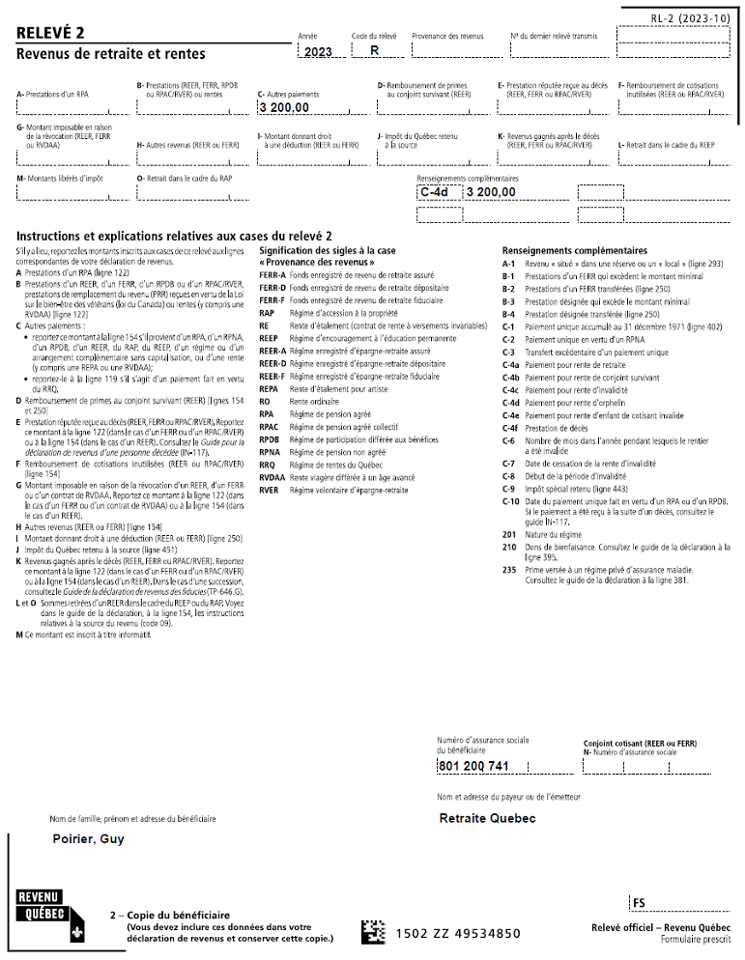
\includegraphics[width=.9\textwidth]{exercice/7-2/Q2/RL2.png}
		\caption[]{Exercice 2, Relevé~2}
		\label{fig:chap7Exercice2RL2}
	\end{figure}
\end{question}
Le Relevé~2 est au nom de Guy Poirier. La case~C-4d du Relevé~2 indique qu'il a reçu des prestations d'orphelin. Il doit déclarer le montant sur ses déclarations T1 ligne~11400 et TP-1 ligne~119.


\begin{question}
	Stéphane Santerre a reçu le T4E(Q), figure~\ref{fig:chap7Exercice2T4EQ}.
	\begin{figure}
		\centering
		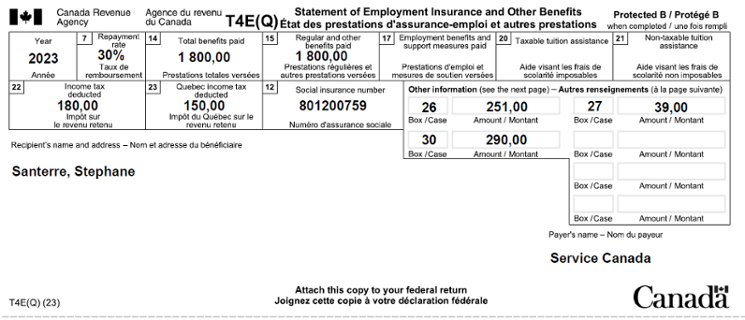
\includegraphics[width=.9\textwidth]{exercice/7-2/Q3/T4EQ.png}
		\caption[]{Exercice 2, T4E(Q)}
		\label{fig:chap7Exercice2T4EQ}
	\end{figure}
\end{question}
\setcounter{sousQuestion}{0}
\begin{sousQuestion}
	Que signifient les montants dans les cases~26, 27 et 30 du feuillet~T4E?
\end{sousQuestion}
Le montant inscrit à la case~26 représente un trop-perçu qui a été recouvré alors que Stéphane percevait des prestations d'assurance-emploi. Il est également inclus dans le montant de la case~30.

Le montant inscrit à la case~27 représente l'annulation de l'impôt retenu pour le montant inscrit à la case~26. Il est également inclus dans le montant de la case~30.

Le montant de la case~30 représente le total des remboursements effectués par Stéphane pendant qu'il percevait les prestations. Ce montant correspond au total des cases~26 et 27.

\begin{sousQuestion}
	Comment traitez-vous ces informations sur les déclarations de Stéphane?
\end{sousQuestion}
Les \numprint{1800}~\$ de prestations versées à Stéphane Santerre doivent être reportées comme revenu aux lignes~11900 de la T1 et 111 de la TP-1. Quant aux 290~\$ qui ont été remboursés, une déduction correspondante peut être réclamée, au fédéral, à la ligne~23200 de la T1, en indiquant qu'il s'agit de prestations d'assurance-emploi remboursées. Au Québec, cette déduction peut être réclamée à la ligne~246 de la TP-1.

\begin{question}
	Le revenu net avant rajustements de Stéphane Santerre (Q3) est de \numprint{77375}~\$.
\end{question}
\setcounter{sousQuestion}{0}
\begin{sousQuestion}
	Quel est le seuil au-dessus duquel il est obligé de rembourser une partie de ses prestations d'assurance-emploi?
\end{sousQuestion}
Le seuil est de \numprint{76875}~\$.

\begin{sousQuestion}
	Calculez le montant du remboursement des prestations d'AE de Stéphane en utilisant la grille du \href{https://www.canada.ca/fr/agence-revenu/services/formulaires-publications/formulaires/t4e.html}{T4E}, cf.~figure~\ref{fig:chap7Exercice2T4E}.
	\begin{figure}
		\centering
		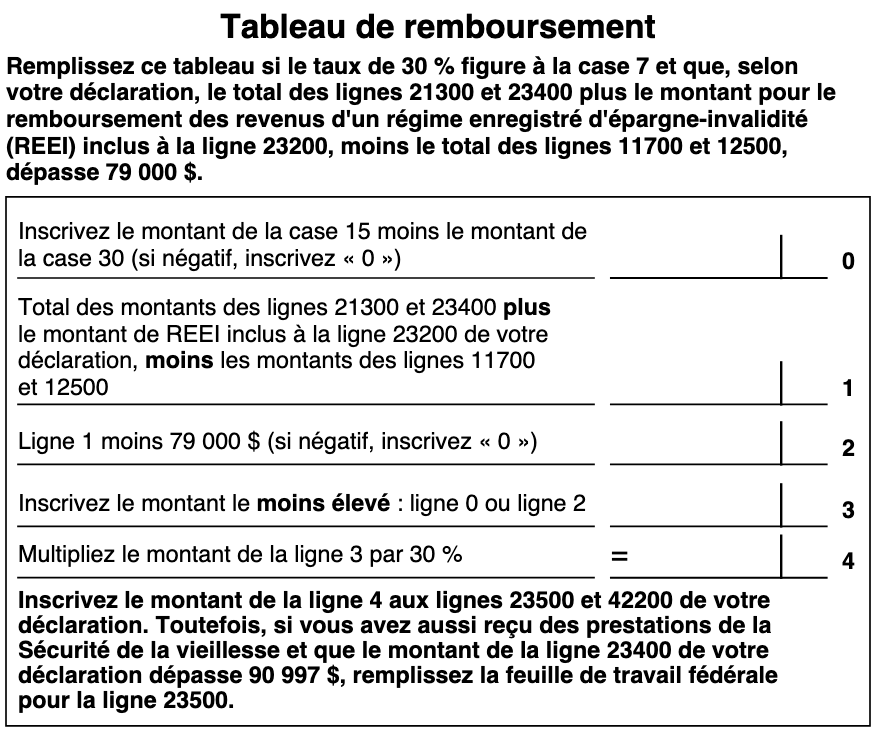
\includegraphics[width=.9\textwidth]{exercice/7-2/Q4/T4E.png}
		\caption[]{Exercice 2, T4E(Q), Tableau de remboursement}
		\label{fig:chap7Exercice2T4E}
	\end{figure}
\end{sousQuestion}
Le remboursement des prestations sociales de Stéphane est de 150~\$, tel que calculé dans la grille de remboursement, cf.~igure~\ref{fig:chap7Exercice2T4ERep}.
\begin{figure}
	\centering
	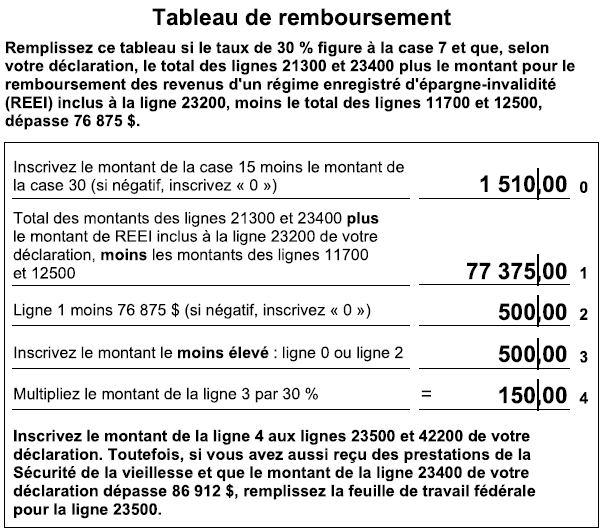
\includegraphics[width=.9\textwidth]{exercice/7-2/Q4/T4EReponse.png}
	\caption[]{Exercice 2, T4E(Q), Tableau de remboursement, rempli}
	\label{fig:chap7Exercice2T4ERep}
\end{figure}
\begin{sousQuestion}
	À quelles lignes de sa T1 et de sa TP-1, ce remboursement doit-il être inscrit? 
\end{sousQuestion}
Au fédéral, le montant doit être inscrit aux lignes~23500 et 42200 de la T1. Au Québec, il doit l'être à la ligne~250, code \og 03\fg{} à la case~249 de la TP-1.



\section{Paiements et remboursements rétroactifs des prestations liées à la COVID-19}
Les programmes d'aide COVID-19 ont pris fin, mais il est toujours possible de recevoir des paiements rétroactifs en 2023. Tous ces avantages sont imposables dans l'année où ils sont reçus, donc tout revenu reçu en 2023 est déclaré sur un feuillet~T4A de 2023 dans l'une des cases suivantes:
\begin{itemize}
	\item case~197: Prestation canadienne d'urgence (PCU);
	\item case~198: Prestation canadienne d'urgence pour les étudiants (PCUE);
	\item case~199: Prestation canadienne d'urgence pour les étudiants (PCUE) pour les étudiants handicapés admissibles ou ceux qui ont des enfants ou d'autres personnes à charge;
	\item case~200: Paiements d'aide financière provinciaux ou territoriaux liés à la COVID-19;
	\item case~202: Prestation canadienne de la relance économique (PCRE);
	\item case~203: Prestation canadienne de maladie pour la relance économique (PCMRE);
	\item case~204: Prestation canadienne de la relance économique pour proches aidants (PCREPA);
	\item case~211: Prestation canadienne pour les travailleurs en cas de confinement (PCTCC).
\end{itemize}

Chacun de ces avantages est déclaré à la ligne~13000 de la déclaration de revenus. Certaines de ces prestations comportaient une retenue d'impôt de 10~\% sur les paiements, mais d'autres n'ont pas retenu d'impôt. Si de l'impôt a été retenu, il est déclaré à la case~022 du feuillet~T4A. 


\subsection{Remboursements des prestations COVID}
De nombreux contribuables ont reçu des prestations auxquelles ils n'avaient pas droit et les ont remboursées par la suite. Si le montant a été reçu et remboursé en 2024, le revenu déclaré sur le feuillet~T4A de 2024 est réduit proportionnellement. Si un revenu a été reçu en 2020 ou 2021 et n'a été remboursé qu'en 2023, il peut être demandé comme déduction dans la déclaration de revenus de 2023. Le remboursement de la prestation liée à la COVID est inscrit comme déduction à la ligne~23200.

Les prestations qui ont été remboursées dans une année différente de celle où elles ont été reçues sont indiquées à la case~201 du feuillet~T4A si les prestations ont été demandées par l'intermédiaire de l'ARC. Si elles ont été demandées par l'intermédiaire de Service Canada, elles sont incluses à la case~30 du feuillet~T4E avec toutes les prestations d'assurance-emploi qui ont été remboursées. Service Canada enverra au bénéficiaire une lettre indiquant le montant lié à la PCU.



\section{Autres revenus}
\begin{intro}
	La plupart des autres revenus, c'est-à-dire les revenus qui n'ont pas à être déclarés à une ligne spécifique des déclarations de revenus, doivent être déclarés à la ligne~13000 de la T1 et à la ligne~154 de la TP-1. Sur cette page, vous verrez des revenus moins communs. La plupart des revenus énumérés ci-dessous sont à inscrire aux lignes~13000 de la T1 et à la ligne~154 de la TP-1 à moins d'indication contraire.
\end{intro}


\subsection{Gains d'un vol ou d'un détournement de fonds}
Tous les montants reçus à la suite d'activités criminelles doivent être inclus dans le revenu. Si les biens reçus sont des biens autres que des espèces, leur juste valeur marchande doit être incluse comme revenu. Si le contribuable rembourse des montants qu'il a inclus auparavant dans son revenu, il peut réclamer une déduction pour le montant remboursé aux lignes~23200 de la déclaration T1 et 250, code \og 17 \fg{} à la case~249, de la déclaration~TP-1.


\subsection{Prestation consécutive au décès}
La prestation consécutive au décès est un montant payé à l'époux ou conjoint de fait, ou à toute autre personne, à la suite du décès d'un employé en reconnaissance des années de services de ce dernier. Au provincial, elle est désignée sous l'appellation \og prestation au décès \fg{} (Ne pas confondre avec la prestation de décès).

Les prestations consécutives au décès sont inscrites aux cases~106 du T4A et O du relevé~1. Au Québec, le code \og RK \fg{} est indiqué à la case Code (case~O) du relevé~1. Elles peuvent aussi être inscrites aux cases~26 du T3 et G du relevé~16.

Les premiers \numprint{10000}~\$ d'une prestation consécutive au décès sont exonérés d'impôt. Cela réduit le montant à déclarer. Cette réduction pouvant aller jusqu'à \numprint{10000}~\$ du montant brut est versée à l'époux(se) ou au conjoint(e) de fait survivant ou à d'autres bénéficiaires. Seul le montant net doit être déclaré à la ligne~13000 de la T1 en spécifiant \og Prestation de décès \fg{} à cette ligne, et à la ligne~154 de la déclaration~TP-1, en utilisant le code 03 à la case~153. 

\subsubsection{Répartition de l'exemption de \numprint{10000}~\$ entre les bénéficiaires}
Au fédéral, lorsqu'il n'y a qu'une seule bénéficiaire, il est relativement facile de calculer le montant qui n'est pas imposable. En effet, on soustrait tout simplement l'exemption de \numprint{10000}~\$ du montant total reçu. Toutefois:

\begin{itemize}
	\item Lorsqu'il y a un(e) conjointe survivant(e) et un autre bénéficiaire ou plus, l'exemption doit être réclamée en premier par la/le conjoint(e) survivant(e) et le reste par les autres personnes.
	\item S'il n'y a aucun(e) conjoint(e) survivant(e) et que des prestations consécutives au décès ont été versées à plus d'une personne, tous les bénéficiaires de la prestation doivent se partager l'exemption maximale, selon la proportion du montant reçu par chacun.
\end{itemize}

Au Québec, l'exemption de \numprint{10000}~\$ doit être répartie proportionnellement aux montants reçus, même si l'un des bénéficiaires de la prestation au décès est le/la conjoint(e) survivant(e).


\subsection{Supplément d'un programme gouvernemental d'incitation au travail}
Il s'agit d'un supplément de revenu que le contribuable a reçu dans le cadre d'un programme gouvernemental d'incitation au travail. Au Québec, les montants sont versés à titre de soutien financier par le ministère de l'Emploi et de la Solidarité sociale. Ils doivent être inclus dans le revenu du bénéficiaire, tant au fédéral qu'au Québec. 

Au fédéral, les montants versés sont inscrits à la case~028 du T4A et reportés à la ligne~13000 de la T1. Au Québec, les sommes versées sont indiquées à la case~O du relevé~1, code \og RS \fg{} à la Code (case~O), et elles sont reportées à la ligne~154, code \og 02 \fg{} à la case~153, de la TP-1.

Le supplément reçu dans le cadre du Programme gouvernemental d'incitation au travail est considéré comme un revenu de travail, au même titre que les montants reçus à titre de traitement ou de salaire, dans:
\begin{itemize}
	\item Le calcul de la déduction pour produits et services de soutien à une personne atteinte d'une déficience, au fédéral et au Québec;
	\item Le calcul de la déduction pour travailleur réclamée au Québec et le calcul du montant canadien pour emploi réclamé au fédéral;
	\item Le calcul du crédit d'impôt pour prolongation de carrière, au Québec.
\end{itemize}


\subsection{Participation à des essais cliniques}
Certaines sociétés pharmaceutiques recrutent des gens via des annonces dans les journaux pour tester des médicaments et versent des indemnités en argent aux participants. Selon l'ARC et Revenu Québec, ces indemnités sont imposables à titre de revenu d'emploi ou d'entreprise, selon le cas.

Au Québec, les premiers \numprint{1500}~\$ d'une indemnité reçue par un participant à des essais cliniques ne sont pas imposables. Une déduction peut donc être réclamée à la ligne~250, code \og 17 \fg{} à la case~249, de la TP-1.

Cette déduction correspond au moins élevée des montants suivants: \numprint{1500}~\$ ou le montant inclus dans le calcul du revenu du contribuable à titre d'indemnité reçue pour sa participation à des essais cliniques. 

Le fédéral n'accorde pas une telle déduction.


\subsection{Allocation canadienne aux parents de jeunes victimes de crimes}
L'allocation canadienne aux parents de jeunes victimes de crimes offre des compensations aux parents qui ont dû s'absenter du travail pour faire face à la mort ou la disparition d'un enfant en raison d'une infraction ou d'une infraction probable au Code criminel.

Les subventions offrent 450~\$ en soutien de revenu par semaine, jusqu'à 35 semaines. Afin d'être admissibles, les parents doivent avoir gagné un minimum de \numprint{6500}~\$ dans l'année civile précédente ou dans les 52 dernières semaines et ont dû s'absenter de leur emploi.

Le montant sera identifié dans la case~136 du T4A et à la case~O du relevé~1 (identifié par le code \og CD \fg{}). Il doit être inclus dans le revenu aux lignes~13000 de la T1 et 154, avec le code 03 à la case~153, de la TP-1.


\subsection{Autres montants}
Les divers montants suivants sont également déclarés aux lignes~13000 de la T1 et 154 de la TP-1.


\subsection{Paiements rétroactifs provenant d'autres sources}
Le contribuable peut choisir que certains paiements rétroactifs provenant de sources soient imposés comme s'ils avaient été reçus dans l'année pour laquelle ils étaient censés être payés.
\begin{itemize}
	\item Les bourses d'études, de perfectionnement ou toute aide financière semblable qui n'est pas exemptée d'impôt;
	\item Les allocations de retraite et de départ;
	\item Les paiements forfaitaires d'un \acrshort{rpa} ou d'un \acrshort{rpdb}; 
	\item Certains paiements reçus d'un \acrfull{reee};
	\item Les sommes reçues en vertu d'une convention de retraite;
	\item Tout autre revenu imposable qui n'est pas inscrit sur une autre ligne.
\end{itemize}



\section{Autres déductions}
\begin{intro}
	Tout remboursement effectué dans l'année d'imposition en cours pour un revenu déclaré au cours de l'année ou des années précédentes peut être réclamé en déduction. Il est possible que ces remboursements réduisent le revenu de l'année précédente au lieu de celui de l'année en cours.
\end{intro}


\subsection{Remboursement de sommes déclarées comme revenu}
Il arrive parfois que certains revenus doivent être remboursés pour diverses raisons (par exemple, non-admissibilité, fraude, etc.). Tout remboursement d'un montant qui a été déclaré comme revenu dans l'année courante ou dans une année antérieure peut être déduit dans l'année du remboursement.

Au fédéral, une déduction peut être réclamée à la ligne~23200 de la T1. Au Québec, elle peut être réclamée à la ligne~246 de la TP-1.

Si le contribuable a reçu un salaire ou des prestations d'assurance salaire durant une période où il n'exerçait pas les fonctions afférentes à son emploi et qu'il a dû les rembourser, ils peuvent être déduits aux lignes~22900 de la T1 et 207, code \og 12 \fg{} à la case~206, de la TP-1. Il faut toutefois que le contribuable les ait inclus dans son revenu pour l'année en cours ou pour une année antérieure. 


\subsection{Déduction ou crédit d'impôt remboursable -- Québec}
Si, en 2023, un contribuable a remboursé un montant qu'il a reçu au cours d'une année antérieure en vertu du RRQ ou du RQAP, il peut demander à Revenu Québec de calculer s'il est plus avantageux pour lui de ne pas utiliser le remboursement pour réduire le revenu de l'année précédente et de se voir plutôt accorder un crédit d'impôt dans l'année courante pour l'étalement de la déduction à la ligne~462 de sa déclaration~TP-1. 

Dans une telle situation, le contribuable doit reporter le montant du remboursement à la ligne~246 de sa TP-1, ainsi à la ligne~462, code \og 08 \fg{} à la case~461. Il doit joindre à sa déclaration provinciale une note précisant l'année visée par le remboursement et les documents justifiant ce remboursement. Revenu Québec accordera le crédit d'impôt, si c'est plus avantageux pour le contribuable.



\section{Frais juridiques}
\begin{intro}
	Un ensemble limité de frais juridiques peut être réclamé à titre de déduction. La raison pour laquelle les frais juridiques ont été encourus détermine sur quelle ligne la déduction peut être réclamée.
\end{intro}

Les frais juridiques suivants peuvent être réclamés à la ligne~22900 de la T1 et à la ligne~207, code \og 09 \fg{} à la case~206, de la TP-1:

\begin{itemize}
	\item Les frais juridiques payés pour percevoir ou établir le droit à un salaire ou un traitement, ou pour établir un droit à ceux-ci. Même si le contribuable ne reçoit aucun montant dans l'année, cela ne l'empêche pas de déduire les frais payés s'il est établi qu'une somme lui est due:
	\begin{itemize}
		\item Le montant admissible à la déduction est le coût payé moins tout parti de ce montant qui a été accordé par le tribunal. Si les frais sont remboursés ou accordés par le tribunal au cours de l'année suivante, ils doivent être ajoutés aux revenus pour l'année où ils ont été reçus;
		\item Un contribuable peut déduire les frais juridiques payés pour recouvrer un montant qui lui est dû ou pour établir un droit à des montants qui, s'il les recevait, seraient inclus dans son revenu d'emploi même s'ils ne sont pas payés directement par son employeur;
	\end{itemize}
	\item Les frais juridiques payés pour percevoir une prestation d'assurance salaire (à laquelle l'employeur contribuait) ou pour établir un droit à celle-ci.
\end{itemize}

Par ailleurs, les frais juridiques suivants sont déductibles à la ligne~23200 de la T1 et 250, code \og 08 \fg{} à la case~249, de la TP-1:

\begin{itemize}
	\item Les frais juridiques payés par le contribuable pour des services de consultation et d'aide (y compris tous les frais comptables connexes) pour répondre à l'ARC et à Revenu Québec lorsqu'ils vérifient ses revenus, déductions ou crédits pour une année donnée;
	\item Les honoraires ou les frais engagés pour préparer, présenter ou poursuivre une opposition ou pour faire appel concernant une cotisation établie ou une décision prise selon la \textbf{Loi de l'impôt sur le revenu}, la \textbf{Loi sur les impôts au Québec}, la \textbf{Loi sur l'assurance-emploi} et le \textbf{Régime de rentes du Québec};
	\item Les frais juridiques payés pour obtenir ou recouvrer une allocation de retraite ou une prestation de retraite ou pour établir un droit à l'une de celles-ci jusqu'à concurrence des sommes reçues dans l'année, moins toute partie de ces montants qui auraient pu être transférés à un régime de retraite;
	\item Toute fraction non déduite peut être reportée aux sept années suivantes.
\end{itemize}


\subsection{Frais juridiques non déductibles}
Les frais juridiques qui ne peuvent pas être réclamés comprennent notamment:
\begin{itemize}
	\item Les frais engagés pour se défendre contre des accusations au civil / criminel;
	\item Les frais engagés pour faire l'acquisition d'une immobilisation (ces frais sont utilisés pour augmenter le prix de base rajusté du bien).
\end{itemize}



\section{Déductions supplémentaires}
\begin{intro}
	Après avoir déterminé le revenu net aux lignes~23600 de la T1 et 275 de la TP-1, le contribuable peut réclamer d'autres déductions lors du calcul de son revenu imposable.
\end{intro}


\subsection{Déduction pour revenu non imposable selon une convention fiscale}
Le contribuable peut réclamer une déduction à la ligne~25600 de la T1 et à la ligne~297, code \og 12 \fg{} à la case~296, de la TP-1 pour un revenu de source étrangère qui est non imposable au Canada selon une convention fiscale. Pour réclamer la déduction, il doit avoir inclus le montant reçu dans ses revenus. Il peut s'agir de revenus étrangers de placement ou de retraite.


\subsection{Vœu de pauvreté perpétuelle}
Au fédéral, le membre d'un ordre religieux qui a prononcé des vœux de pauvreté perpétuelle peut donner son revenu gagné et son revenu de pension à cet ordre. Par contre, il peut réclamer une déduction correspondante à la ligne~25600 de sa T1.

Pour avoir droit à cette déduction, le contribuable doit avoir donné tout revenu gagné à l'ordre religieux et non seulement une partie de celui-ci. Ceci remplace le crédit pour dons de bienfaisance qui est discuté plus loin dans ce chapitre. Il doit joindre une lettre de sa communauté ou de son employeur attestant son vœu de pauvreté perpétuelle. 

Il n'y a pas de déduction équivalente pour le Québec. 


\subsection{Aide visant les frais de scolarité pour la formation de base des adultes}
Un contribuable qui a inclus dans ses revenus une aide financière pour couvrir une partie ou la totalité des frais de scolarité qu'il a payés pour suivre des cours de niveau primaire ou secondaire peut réclamer une déduction pour le montant de l'aide reçue. 

Cette aide figure à la case~21 de son T4E et elle est incluse dans le montant de la case~14. Cette déduction peut être réclamée à la ligne~25600 de la déclaration T1 et à la ligne~295 de la déclaration~TP-1. 


\subsection{Déductions spécifiques au Québec}
Les déductions suivantes peuvent être réclamées à la ligne~297 de la TP-1: voir table~\ref{table:deductionsSupplementairesSpecifiquesAuQuebec}.
\begin{table}
	\centering
	\begin{tabular}{|l|c|c|}
		\hline
		\multicolumn{3}{|c|}{La déduction s'inscrit à la ligne~297 de la TP-1}                                      \\
		\multicolumn{3}{|c|}{Le code s'inscrit à la case~296}                                                       \\
		\multicolumn{3}{|c|}{Le taux d'exemption se trouve à la case~A-14 du RL-1 (s'il y a lieu)}                  \\ \hline
		\textbf{Description}                                     & \textbf{Code} &      \textbf{Montant de la}      \\
		                                                         & \textbf{case} &     \textbf{déduction à la}      \\
		                                                         & \textbf{296}  &      \textbf{case~Du RL-1}       \\ \hline
		Déduction pour chercheur étranger*                       &      03       &               A-10               \\ \hline
		Déduction pour expert étranger*                          &      04       &               A-12               \\ \hline
		Déduction pour chercheur étranger en stage postdoctoral* &      05       &               A-11               \\ \hline
		Déduction pour spécialiste étranger*                     &      06       &               A-9                \\ \hline
		Déduction pour revenu d'emploi gagné sur un navire       &      08       &               A-6                \\ \hline
		Déduction pour professeur étranger                       &      19       &               A-13               \\ \hline
		Déduction pour le personnel des Forces canadiennes et    &      23       &               A-7                \\
		des forces policières                                    &               &                                  \\ \hline
		Déduction pour remboursement d'une prestation            &      24       &             case~12              \\
		universelle pour garde d'enfants                         &               &             du RC62              \\ \hline
		Déduction pour remboursement d'une prestation d'un       &      25       &              s. o.               \\
		régime enregistré d'épargne-invalidité                   &               &                                  \\ \hline
		\multicolumn{3}{|l|}{*La déduction disponible doit être réduite de la somme des montants des cases~105,}    \\
		\multicolumn{3}{|l|}{205 et 207 associés aux revenus admissibles à cette déduction, multipliée par le taux} \\
		\multicolumn{3}{|l|}{de la case~A-14.}                                                                      \\ \hline
	\end{tabular}
	\caption{Déductions supplémentaires spécifiques au Québec}
	\label{table:deductionsSupplementairesSpecifiquesAuQuebec}
\end{table}

\rqg[s]{47 à 49}



\section{Achat d'une habitation}
\begin{intro}
	Les acheteurs d'une première maison peuvent réclamer un crédit d'impôt non remboursable d'un montant de \numprint{10000}~\$ (augmentation de \numprint{5000}~\$ par rapport à 2023) pour l'achat d'une habitation admissible qu'ils ont acquise dans l'année d'imposition.
\end{intro}

Pour réclamer le crédit d'impôt, les conditions suivantes doivent être respectées:
\begin{itemize}
	\item Le contribuable ou sa conjointe (épouse ou de fait) a fait l'acquisition d'une habitation admissible; 
	\item Le contribuable n'a pas habité, au cours de l'année d'acquisition ou des quatre années précédentes, dans une autre habitation dont lui-même ou sa conjointe (épouse ou de fait) était propriétaire;
	\item Le contribuable sera admissible au crédit d'impôt si sa conjointe (épouse ou de fait) était propriétaire d'une habitation pendant la période en question. Toutefois, le contribuable ne peut y avoir vécu pendant qu'ils étaient mariés ou en union de fait.
\end{itemize}

Une \og habitation admissible \fg{} comprend les maisons unifamiliales, les maisons semi-détachées, les maisons en rangée, les maisons mobiles, les habitations en copropriété (condominiums), les appartements dans un duplex, un triplex, un quadruplex ou un immeuble, et les parts dans une coopérative d'habitation en tant que propriétaire. Il peut s'agir aussi d'une habitation existante ou en construction.

Cette habitation doit être située au Canada et enregistrée au nom du contribuable et à celui de son époux(se) ou conjoint(e) de fait.

Les documents justificatifs doivent inclure:
\begin{itemize}[label=\twemoji{check box with check}]
	\item Le nom de l'acheteur;
	\item La date de clôture de la transaction;
	\item L'adresse de la propriété;
	\item Si l'habitation est achetée pour une personne handicapée;
	\item La date d'acquisition de l'habitation.
\end{itemize}

Les époux ou conjoints de fait peuvent se partager le montant entre eux quel que soit le nom qui figure sur l'enregistrement de la maison. Si plus d'une personne a droit au montant, le montant total que les personnes peuvent réclamer pour l'année ne doit pas dépasser le montant total du crédit.

Le montant pour l'achat d'une habitation peut aussi être réclamé à l'égard de certaines habitations acquises par les personnes admissibles au crédit d'impôt pour personnes handicapées ou au bénéfice de ceux-ci si l'acquisition leur permet de vivre dans une habitation plus accessible ou dans un environnement mieux adapté à leurs besoins personnels et leurs soins. Un contribuable n'a pas à être l'acheteur d'une première habitation s'il a droit au montant pour personnes handicapées ou s'il fait l'acquisition d'une habitation au bénéfice d'un parent qui y a droit.


\subsection{Le crédit d'impôt}
Le crédit d'impôt non remboursable pour l'achat d'une habitation est de \numprint{10000}~\$ au fédéral et de \numprint{10000}~\$ au Québec.

Au fédéral, le crédit d'impôt de \numprint{10000}~\$ s'inscrit à la ligne~31270 de la T1. Bien entendu, le taux de 15~\% sera appliqué pour obtenir un crédit d'impôt net de \numprint{1500}~\$.

Au Québec, le crédit d'impôt est calculé sur le formulaire TP-752.HA. Le crédit d'impôt maximum résultant de ce calcul est de \numprint{1500}~\$. Ce montant sera inscrit à la ligne~396 de la TP1.

\qct\href{https://www.revenuquebec.ca/fr/services-en-ligne/formulaires-et-publications/details-courant/tp-752-ha/}{TP-752.HA -- Crédit d'impôt pour achat d'une habitation}

\subsubsection{Informations supplémentaires pour la TP-1}
Contrairement à la réclamation fédérale sur la T1, le contribuable ne peut pas simplement réclamer \numprint{1500}~\$ ou sa part du crédit.

Dans le calcul dans le TP.752.HA, le montant qui peut être réclamé dépend de la différence entre l'impôt sur le revenu imposable à la ligne~401 moins la somme des crédits non remboursables des lignes~359 à 367 multipliée par 15~\% moins les montants demandés aux lignes~391 et 397.

En effet, le montant du crédit d'impôt pour l'achat d'une habitation est limité au montant requis pour réduire l'impôt sur le revenu imposable à zéro ou jusqu'au maximum de \numprint{1500}~\$.

Si le contribuable dispose déjà de suffisamment de crédits non remboursables pour réduire à zéro l'impôt sur le revenu imposable, aucun crédit d'impôt pour achat d'une habitation ne sera accordé.

Il est donc possible que le contribuable ne puisse pas réclamer sa juste part du crédit.

Par conséquent, ils devraient envisager de laisser à l'autre co-acheteur une plus grande part des \numprint{1500}~\$ si cela est plus efficace sur le plan fiscal pour eux.



\section{Nouvelles numériques}
\begin{intro}
	Un contribuable admissible qui a payé des frais pour un abonnement aux nouvelles numériques à une organisation journalistique canadienne qualifiée peut réclamer un crédit d'impôt non remboursable pour les montants engagés.
\end{intro}

Il s'agit d'un crédit temporaire admissible sur la T1 pour les années d'imposition de 2020 à 2024. Le contribuable ne peut pas réclamer plus de 500~\$ et doit être inscrit à la ligne~31350 de la T1.

Afin d'être admissible au crédit, l'abonnement doit être fait à une \og \acrfull{ojcq} \fg{} qui se consacre principalement à la production de contenu original de nouvelles écrites. Les organismes engagés de quelque manière que ce soit dans la radiodiffusion ne seront pas admissibles.

\cat\href{https://www.canada.ca/fr/agence-revenu/services/impot/particuliers/sujets/tout-votre-declaration-revenus/declaration-revenus/remplir-declaration-revenus/deductions-credits-depenses/toutes-deductions-tous-credits-toutes-depenses/abonnement-aux-actualites-numeriques/liste-abonnements-nouvelles-numeriques-admissibles.html}{Liste des abonnements aux nouvelles numériques admissibles}

La définition d'une OJCQ est longue et technique. Cependant, il y a trois conditions particulièrement importantes:
\begin{itemize}
	\item Son contenu doit être édité et conçu au Canada;
	\item Elle doit être principalement engagée dans la production de contenus d'actualités originaux qui:
	\begin{itemize}
		\item Doit être principalement axé sur des questions d'intérêt général et des rapports sur l'actualité, y compris la couverture des institutions et processus démocratiques, et
		\item Ne doit pas être principalement axé sur un sujet particulier comme des nouvelles spécifiques à l'industrie, les sports, les loisirs, les arts, le style de vie ou le divertissement.
	\end{itemize}
	\item Elle n'est pas engagée de manière significative dans la production de contenu qui:
	\begin{itemize}
		\item Fait la promotion des intérêts ou rend compte des activités d'une organisation, d'une association ou de ses membres,
		\item Est produit pour un gouvernement, une société d'État ou un organisme gouvernemental, ou
		\item Fais la promotion de biens et services.
	\end{itemize}
\end{itemize}



\section{Dons}
\begin{intro}
	Un contribuable qui fait un don d'argent ou de biens à des organismes de bienfaisance enregistrés peut avoir droit à un crédit d'impôt non remboursable pour ce don, au fédéral et au Québec. Il peut ainsi réclamer le montant admissible d'un don qu'il a fait en 2023 et au cours des années 2018 à 2022, s'il n'a jamais réclamé de crédit pour ces derniers.
\end{intro}


\subsection{Don de bienfaisance}
Le crédit d'impôt, pour un don justifié par un reçu officiel, s'inscrit à la ligne~34900 de la T1 et à la ligne~395 de la TP-1. 

Au fédéral, le montant admissible des dons ne doit pas dépasser 75~\% du revenu net (ligne~23600 de la T1). Au Québec, il n'y a pas de limite.

\subsubsection{Reçu et montant admissible d'un don}
Un reçu pour don doit porter le nom de l'organisme de bienfaisance ainsi que son numéro d'entreprise, lequel a été obtenu auprès de l'ARC ou de Revenu Québec. Le nom et l'adresse complète du donateur doivent aussi y être clairement indiqués. De plus, le reçu doit être signé par un responsable dûment autorisé de l'organisme de charité, et il doit être numéroté.

Au fédéral seulement, le reçu doit porter le nom \og Agence de revenu du Canada \fg{}, qu'il soit écrit à la main ou au moyen d'un autocollant ou d'une estampe. Le reçu doit également indiquer le \og montant admissible \fg{} du don. 

Le don prélevé à la source par l'employeur apparaît aux cases~46 et N des T4 et relevé~1. Aucun reçu officiel requis.

Un don peut aussi être prélevé:
\begin{itemize}
	\item À la case~46 du T4A et à la case~210 du relevé~2;
	\item À la case~48 du T3 et à la case~N du relevé~16;
	\item Aux cases~182 et 183 du T5013 et aux cases~19 et 20 du relevé~15;
	\item À la case~13 du T5003 et à la case~H du relevé~14.
\end{itemize}

Le contribuable doit conserver ses reçus de dons pour éléments de preuve.

Dans ce cours, nous nous concentrons sur les dons en argent plutôt que sur les dons en nature qui sont plus complexes pour déterminer le traitement fiscal.

Il est possible que certains organismes prétendent être des organismes de bienfaisance. S'ils ne sont pas enregistrés auprès de l'ARC, un crédit d'impôt ne peut être réclamé.

\cat\href{https://apps.cra-arc.gc.ca/ebci/hacc/srch/pub/dsplyBscSrch}{Liste des organismes de bienfaisance et de certains autres donataires reconnus -- Recherche de base}


\subsection{Dons admissibles}
Courte liste d'organismes de bienfaisance enregistrés:
\begin{itemize}
	\item La Société canadienne de la croix rouge;
	\item Centraide;
	\item La Société canadienne du cancer;
	\item L'Armée du salut;
	\item Le YMCA et le YWCA;
	\item Les scouts et les guides;
	\item Les églises, temples, synagogues et autres;
	\item La Fondation canadienne des maladies du cœur et autres fondations;
	\item Les écoles sans but lucratif, les collèges, les universités, les bibliothèques et les musées.
\end{itemize}

Un don octroyé à une école réservée à l'instruction religieuse, à une école autre qu'un établissement postsecondaire ou un établissement scolaire désigné est admissible comme don de charité, mais non comme frais de scolarité. Le don octroyé pour l'enseignement religieux dans des institutions d'enseignement primaire et secondaire est admissible au fédéral seulement.

\begin{note}
	La catégorie d'\acrfull{oje} a été ajoutée pour 2020. Au Québec, deux OJE:
	\begin{itemize}
		\item La Presse inc.: média numérique indépendant dont la mission est d'offrir une information de qualité, gratuite et accessible à tous;
		\item Journaldesvoisins.com: journal indépendant, communautaire, professionnel et quotidien d'informations locales.
	\end{itemize}
\end{note}

\subsubsection{Dons admissibles seulement au Québec}
Au Québec seulement, un contribuable peut réclamer:
\begin{itemize}[label=\twemoji{check mark button}]
	\item Le don offert à un organisme d'éducation politique ou à un organisme artistique reconnu par le Ministre du Revenu du Québec;
	\item Le don offert à l'Agence de la Francophonie ou à l'un de ses organismes subsidiaires;
	\item Le don d'un instrument de musique, offert après le 23 mars~2006, à un établissement d'enseignement reconnu;
	\item Le don de biens culturels offert au Musée national des beaux-arts du Québec, au Musée d'Art contemporain de Montréal et au Musée de la civilisation;
	\item Le don d'une denrée alimentaire offert par une entreprise agricole.
\end{itemize}


\subsection{Dons non admissibles}
\begin{itemize}[label=\twemoji{cross mark}]
	\item Le don fait à des organisations de bienfaisance hors du Canada, sauf aux organisations désignées par les gouvernements;
	\item Le don fait à un contribuable;
	\item La valeur des services rendus;
	\item La valeur des marchandises dont le coût est imputé à une dépense d'entreprise 
	\item Le don de vêtements, mobiliers ou autres, à un organisme non enregistré;
	\item Le montant payé pour des billets à l'occasion de parties de cartes, bingos, loteries ou autres;
	\item Le don fait aux organisations patriotiques, fraternelles ou de secours mutuels; ou
	\item Au Québec, le don pour l'enseignement religieux.
\end{itemize}


\subsection{Traitement fiscal}
Au fédéral, le crédit d'impôt est calculé sur l'annexe~9 - Dons, avant d'être reporté à la ligne~34900 de la T1.

Le crédit d'impôt pour une année d'imposition donnée est égal au total des montants suivants:
\begin{itemize}
	\item 15~\% sur la première tranche de 200~\$ de dons effectués dans l'année;
	\item 33~\% du moindre:
	\begin{itemize}
		\item Total des dons effectués dans l'année qui excèdent la première tranche de 200~\$,
		\item Revenu imposable de l'année qui excède le seuil du taux d'imposition supérieur des particuliers (\numprint{235675}~\$ en 2023);
	\end{itemize}
	\item 29~\% du total des dons effectués dans l'année, supérieurs à 200~\$ qui ne sont pas admissibles au taux de 33~\% mentionné ci-dessus.
\end{itemize}

Pour la TP-1, le contribuable doit utiliser la grille de calcul de la ligne~395 pour les dons monétaires au cours de l'année. Sinon, l'annexe~V doit être utilisée.

Le crédit d'impôt pour une année d'imposition donnée est égal au total des montants suivants:
\begin{itemize}
	\item 20~\% sur la première tranche de 200~\$ de dons effectués dans l'année;
	\item 25,75~\% du moindre:
	\begin{itemize}
		\item Total des dons effectués dans l'année qui excèdent la première tranche de 200~\$,
		\item Revenu imposable de l'année qui excède le seuil du taux d'imposition supérieur des particuliers (\numprint{119910}~\$ en 2023);
	\end{itemize}
	\item 24~\% du total des dons effectués dans l'année, supérieurs à 200~\$ qui ne sont pas admissibles au taux de 25,75~\% mentionné ci-dessus.
\end{itemize}


\subsection{Report des dons de bienfaisance}
Si les dons de bienfaisance ou autres dons ne réduisent pas à zéro l'impôt à payer, l'excédent peut être reporté sur les cinq années suivantes, sauf les dons de biens écosensibles et de biens culturels attestés faits après le 10~février~2014 sur 10~ans. En raison du délai de cinq ans, le report des années antérieures devrait être appliqué en premier lieu. Une note doit être jointe aux déclarations si le montant a été reporté d'une année précédente.


\subsection{Dons faits par l'époux ou le conjoint de fait}
L'une ou l'autre des personnes dans un couple marié ou en union de fait peut utiliser le reçu, peu importe à qui le reçu est établi. Les dons faits par les époux ou conjoints de fait peuvent être regroupés, afin de les réclamer sur une seule déclaration.

\subsection{Dons de biens}
Les dons de biens autres que l'argent peuvent être réclamés, pourvu qu'ils aient une certaine valeur. Par exemple, les dons de vieux vêtements ne sont pas admissibles puisqu'ils ont peu de valeur. 

\subsubsection{Dons de biens culturels}
Un bien culturel est:
\begin{itemize}
	\item Un bien canadien certifié par la \acrfull{cceebc}. La valeur du bien est inscrite sur le certificat T871, \textbf{Certificat fiscal visant des biens culturels}, émis par cet établissement; 
	\item Un bien québécois reconnu ou classé conformément à la \textbf{Loi sur le patrimoine culturel} ou à la Loi sur les biens culturels;
	\item Un bien pour lequel une \textbf{Attestation d'aliénation de biens culturels} (TPF-712.0.1) a été délivrée par le Conseil du patrimoine culturel du Québec, anciennement appelé Commission des biens culturels du Québec.
\end{itemize}

Pour être reconnu comme don de biens culturels, le don doit être fait à une administration publique ou un établissement prescrit. Le reçu officiel émis par le donataire ainsi que le certificat T871 ou l'attestation doivent être joints aux T1 et TP-1.

Une œuvre d'art créée par un artiste et comprise dans son inventaire, qui est offerte en donation, est un bien culturel. La juste valeur marchande de l'œuvre d'art en question, telle que déterminée par la CCEEBC, représente la valeur du don qui peut être réclamée.

Les dons de biens culturels attestés faits après le 10 février~2014, la juste valeur marchande du bien donné est réputée être le moins élevé des montants suivants:
\begin{itemize}
	\item La JVM déterminée du bien;
	\item Son coût immédiatement avant que le don soit fait.
\end{itemize}

Le montant admissible doit être inscrit à la ligne~34200 de l'annexe~9 (au fédéral) et à la partie 2 de l'annexe~V (au Québec). Le montant pouvant être réclamé n'est pas limité à un pourcentage du revenu net du contribuable (montant de la ligne~23600 de la T1 et du montant de la ligne~275 de la TP-1). 

\subsubsection{Dons d'une œuvre d'art au Québec}
Le don d'une œuvre d'art à un organisme de bienfaisance non relié au domaine des arts n'est admissible au crédit qu'au moment où l'organisme vend l'œuvre en question. La vente doit avoir lieu avant la fin de la cinquième année civile qui suit l'année du don.

C'est donc au moment de la disposition du bien que l'organisme en question remettra un reçu officiel et que le contribuable pourra réclamer le crédit. Si un reçu lui est délivré après la production de sa déclaration~TP-1, le contribuable doit faire une demande de redressement.

La mesure concernant la disposition du bien ne s'applique pas au don d'une œuvre d'art fait:
\begin{itemize}[label=\twemoji{cross mark}]
	\item au gouvernement fédéral, à une province, à une municipalité canadienne;
	\item à un organisme artistique reconnu par Revenu Québec;
	\item à un organisme qui a acquis l'œuvre d'art dans le cadre de sa mission première, aux dons de biens culturels et aux dons ayant une valeur patrimoniale.
\end{itemize}

Si le don d'une œuvre d'art a été fait à un musée situé au Québec ou à une institution muséale reconnue, le montant admissible du don est égal à 125~\% du montant servant au calcul du crédit.

\subsubsection{Dons d'une œuvre d'art public}
Afin d'inciter davantage les contribuables québécois à donner des œuvres d'art destinées à être installées à demeure dans des espaces publics ou des lieux réservés à l'enseignement, le montant admissible du don peut être majoré aux fins du calcul du crédit d'impôt pour dons sur la TP-1. Le don d'une œuvre d'art public doit être fait après le 3~juillet~2014.

Une \og œuvre d'art public \fg{} est une œuvre d'art à caractère permanent, souvent de grande dimension ou de type environnemental, installée dans un espace accessible à la population dans un but de commémoration, d'embellissement des lieux ou encore d'intégration à l'architecture ou à l'environnement de bâtiments et de sites à vocation publique.

Le crédit est augmenté de 25~\% à l'égard d'un don fait au gouvernement du Québec, à un organisme public ou à une municipalité québécoise. Le montant est majoré de 50~\% si l'œuvre acquise est installée dans un lieu d'enseignement situé au Québec.

La majoration du montant admissible d'un don d'une œuvre d'art public est calculée à la partie~A de l'annexe~V (lignes~6 et 8 dans le cas d'un don de bienfaisance et lignes~25 et 27 dans le cas d'un bien culturel).

\subsubsection{Dons de biens écosensibles}
Les dons de terrains, ou servitudes grevant un terrain, qui ont une valeur écologique reconnue par le ministre de l'Environnement, peuvent être admissibles, pourvu que le ministre fédéral de l'Environnement (et le ministère de l'Environnement du Québec pour un fonds de terre situé au Québec) ait certifié que la terre est vulnérable sur le plan environnemental et qu'il est important de la préserver et de la conserver pour protéger le patrimoine environnemental du Canada. Le montant peut être réclamé à la ligne~34200 de l'annexe~9 et à la ligne~22 de l'annexe~V. Il n'est pas limité à un pourcentage du revenu net.

Les dons de biens écosensibles peuvent être reportés jusqu'à 10 ans pour les dons faits à compter du 11~février~2014.

Au fédéral, depuis le 21~mars~2017, les dons de fonds de terre écosensibles ne sont plus admissibles au crédit d'impôt pour dons de bienfaisance, s'ils sont faits à une fondation privée. Ils continueront à être admissibles s'ils sont versés à un organisme de bienfaisance enregistré ou à d'autres donataires reconnus.

\subsubsection{Dons de denrées alimentaires au Québec}
Le montant admissible d'un don fait, après le 26~mars~2015, par un producteur agricole reconnu à un organisme de bienfaisance enregistré qui est soit Les Banques Alimentaires du Québec, soit un membre Moisson, peut être majoré de 50~\% aux fins du calcul de la déduction pour dons ou du crédit d'impôt non remboursable pour dons, selon le cas, si le don porte sur des produits agricoles admissibles.

Producteur agricole reconnu est une personne:
\begin{itemize}
	\item Sois qui exploite une entreprise enregistrée auprès du \acrfull{mapaq} à titre d'exploitation agricole;
	\item Soit un particulier membre d'une société de personnes qui exploite une telle entreprise et qui est membre de la société à la fin de son exercice financier.
	\item 
\end{itemize}

Produit alimentaire admissible:
\begin{itemize}[label=\twemoji{check mark button}]
	\item Viande ou sous-produit de viande;
	\item Œuf;
	\item Produits laitiers;
	\item Fruits;
	\item Légumes;
	\item Céréales;
	\item Légumineuses;
	\item Fines herbes;
	\item Miel;
	\item Sirop d'érable;
	\item Champignons;
	\item Noix;
	\item Etc.
\end{itemize}

\begin{note}
	Un produit transformé n'est pas admissible, sauf si sa transformation n'empêche pas qu'il soit légalement vendu, distribué ou mis en vente en dehors du lieu où il est produit, en tant que produit alimentaire ou boisson destinée à la consommation humaine.
\end{note}

Le contribuable qui a fait un don de denrées alimentaires qu'il transforme, après le 17~mars~2016, peut aussi demander un crédit d'impôt non remboursable pour dons. Le montant admissible de ce don peut être augmenté de 50~\% si, au moment du don, toutes les conditions suivantes étaient remplies:
\begin{itemize}
	\item Il exploite une entreprise de transformation d'aliments;
	\item Le don a été fait à un organisme de bienfaisance enregistré qui était Les Banques alimentaires du Québec, un membre Moisson ou un membre Associé;
	\item Les denrées alimentaires étaient des produits alimentaires admissibles.
\end{itemize}

Le montant peut être réclamé à la ligne~395 de la TP-1. Le contribuable doit remplir l'annexe~V.

\subsubsection{Crédit additionnel pour don important en culture -- Québec}
En plus du crédit d'impôt régulier pour dons de bienfaisance et autres dons calculés à la partie~A de l'annexe~V, un particulier peut avoir droit pour le même don à un crédit d'impôt additionnel pour don important en culture. Ce crédit est disponible si, après le 3~juillet~2013 et avant le 1\ier{}~janvier~2023, il a fait un don en argent d'au moins \numprint{5000}~\$ (effectué en un ou plusieurs versements) à l'un des donataires suivants:
\begin{itemize}
	\item Un organisme de bienfaisance enregistré œuvrant au Québec dans le domaine des arts ou de la culture;
	\item Un organisme culturel ou de communication enregistrée;
	\item Une institution muséale enregistrée, le Musée national des beaux-arts du Québec, le Musée d'art contemporain de Montréal, le Musée de la civilisation ou un musée qui est situé au Québec et constitué en vertu de la Loi sur les musées.
\end{itemize}

Le crédit additionnel est égal à 25~\% du montant admissible du don, jusqu'à l'occurrence d'un don de \numprint{25000}~\$. Il ne peut être réclamé qu'une seule fois. Il est calculé à la partie~B de l'annexe~V.

\subsubsection{Crédit pour dons de mécénat culturel -- Québec}
Un particulier peut demander un crédit d'impôt de 30~\% pour un don en argent d'au moins \numprint{250000}~\$ fait après le 3~juillet~2013 à un donataire admissible. Il s'agit des mêmes donataires qui sont reconnus aux fins du crédit d'impôt additionnel pour don important en culture. Le crédit est admissible même si le versement s'échelonne sur une période d'au plus dix ans, pourvu qu'un minimum de \numprint{25000}~\$ de dons soit fait par année et qu'une promesse de dons est enregistrée auprès du ministre de la Culture et des Communications.

Le crédit est calculé à la partie~C de l'annexe~V. 

Il ne s'agit pas d'un crédit supplémentaire. Ainsi, un contribuable ne pourra pas bénéficier du crédit d'impôt pour dons de bienfaisance et autres dons de la partie~A ni du crédit d'impôt additionnel pour don important en culture pour un don inscrit à la partie~C.

\subsection{Membres d'un ordre religieux}
Au fédéral, comme mentionné précédemment, les membres d'un ordre religieux qui ont prononcé des vœux de pauvreté perpétuelle peuvent donner tout leur revenu gagné à leur ordre. Par contre, ils peuvent réclamer une déduction de ce même montant à la ligne~25600 de leur T1 sans être restreints à la limite du revenu net. Tout leur revenu gagné doit être donné à cet ordre et non seulement une partie de celui-ci. Ils peuvent choisir de réclamer la déduction ou le crédit d'impôt non remboursable.

Au Québec, les membres d'un ordre religieux ayant fait vœu de pauvreté perpétuelle peuvent inscrire comme dons de bienfaisance les sommes remises à leur communauté religieuse jusqu'à concurrence de leur revenu net. 



\section{Exercice 3}
\setcounter{question}{0}
\begin{question}
	Suite au décès de son époux, Marjolaine a reçu \numprint{17000}~\$ de prestations consécutives au décès.
	
	À quelles lignes des déclarations doit-elle inscrire ces prestations? Quel montant doit-elle y inscrire?
\end{question}
Marjolaine doit inscrire \numprint{7000}~\$ (\numprint{17000}~\$ $–$ \numprint{10000}~\$) et \og Prestation consécutive au décès \fg{} à la ligne~13000 de sa T1; et à la ligne~154, code \og 03 \fg{} à la case~153, de sa TP-1.

\begin{question}
	En mars de l'année d'imposition, Micheline Latour a reçu un paiement forfaitaire rétroactif de \numprint{23000}~\$ de son plan de perte d'emploi, dont \numprint{10000}~\$ se rapporte à l'année précédente. Elle n'a jamais cotisé au régime.
\end{question}
\setcounter{sousQuestion}{0}
\begin{sousQuestion}
	Quel montant devrait-elle déclarer dans ses déclarations de revenus fédérale et provinciale pour l'année d'imposition en cours et sur quelles lignes?
\end{sousQuestion}
Micheline doit déclarer \numprint{23000}~\$ à la ligne~10400 de sa T1 et à la ligne~107 de sa TP1, en utilisant le code 02 à la case~106.

\begin{sousQuestion}
	Que doit-elle faire pour s'assurer que les \numprint{10000}~\$ relatifs à une année d'imposition précédente ne sont pas imposables dans l'année d'imposition en cours?
\end{sousQuestion}
Micheline peut demander à l'ARC et à RQ de calculer s'il est plus avantageux pour elle de reporter les \numprint{10000}~\$ à l'année d'imposition précédente. Elle doit faire la demande fédérale en joignant le formulaire T1198 à sa T1. Au Québec, elle doit cocher la case~404 de sa TP-1 et joindre le formulaire TP-766.2 à sa déclaration provinciale.

\begin{question}
	Bernard a payé des frais juridiques de 400~\$ afin de poursuivre son ancien employeur dans le but de récupérer \numprint{2000}~\$ de salaire non payé.
\end{question}
\setcounter{sousQuestion}{0}
\begin{sousQuestion}
	Il a gagné sa cause. En plus de récupérer le salaire qui lui est dû, le jugement de la cour lui a accordé 250~\$ pour couvrir une partie des frais juridiques payés.
	
	Quel montant peut-il déduire à titre de frais juridiques?
\end{sousQuestion}
Il peut déduire 150~\$, soit 400~\$ $-$ 250~\$.

\begin{sousQuestion}
	Si Bernard ne gagne pas sa cause et ne réussit pas à établir qu'un montant lui est dû, quel montant peut-il déduire à titre de frais juridiques au fédéral et au Québec?
\end{sousQuestion}
Même si Bernard ne gagne pas sa cause et ne parvient pas à établir que son employeur lui doit de l'argent, il peut déduire tous ses frais juridiques au Québec, mais pas au fédéral.

\begin{question}
	Indiquez si les dons énumérés ci-dessous sont des dons de bienfaisance admissibles ou non admissibles:
	\begin{enumerate}[label=\Alph*{}.]
		\item Don à la Société canadienne de la Croix-Rouge 	
		\item Don à une personne dans le besoin 	
		\item Don de vieux vêtements à un voisin 	
		\item Don au YMCA ou YWCA de la région 	
		\item Montant payé pour un bingo à l'église 	
		\item Don à l'église locale 	
		\item Don à un organisme religieux enregistré
	\end{enumerate}
\end{question}
\begin{enumerate}[label=\Alph*{}.]
	\item Admissible
	\item Non admissible
	\item Non admissible
	\item Admissible
	\item Non admissible
	\item Admissible
	\item Admissible
\end{enumerate}

\begin{question}
	Jean possède les reçus suivants pour les dons de bienfaisance en argent qu'il a offerts durant l'année d'imposition: table~\ref{table:chap7ex3Q5}.
	\begin{table}
		\centering
		\begin{tabular}{lcr}
			\textbf{Don}                 & \textbf{Date} &   \textbf{Montant} \\ \hline\hline
			Église interconfessionnelle  &     26-07     & \numprint{1700} \$ \\ \hline
			Société canadienne du cancer &     05-08     &             100 \$ \\ \hline
			Université de Montréal       &     02-09     &             150 \$ \\ \hline
			UNESCO                       &     16-10     &             200 \$ \\ \hline
			Scout Québec                 &     19-10     &              50 \$ \\ \hline
			Total des dons               &     31-12     & \numprint{2200} \$ \\ \hline
		\end{tabular}
		\caption[]{Exercice 3, dons}
		\label{table:chap7ex3Q5}
	\end{table}
	
	Ses revenus net et imposable au fédéral et Québec sont de \numprint{235908}~\$. Il désire réclamer le maximum au titre des dons de bienfaisance sur sa déclaration fédérale pour l'année d'imposition courante. C'est la première fois qu'il distribue des dons et qu'il réclame le crédit d'impôt. 
\end{question}
\setcounter{sousQuestion}{0}
\begin{sousQuestion}
	Complétez l'\href{https://www.canada.ca/fr/agence-revenu/services/formulaires-publications/trousses-impot-toutes-annees-imposition/trousse-generale-impot-prestations/5000-s9.html}{annexe~9}.
\end{sousQuestion}
Jean peut demander un crédit d'impôt de 619,32~\$, cf. figure~\ref{fig:chap7Exercice3Annexe9}.
\begin{figure}
	\centering
	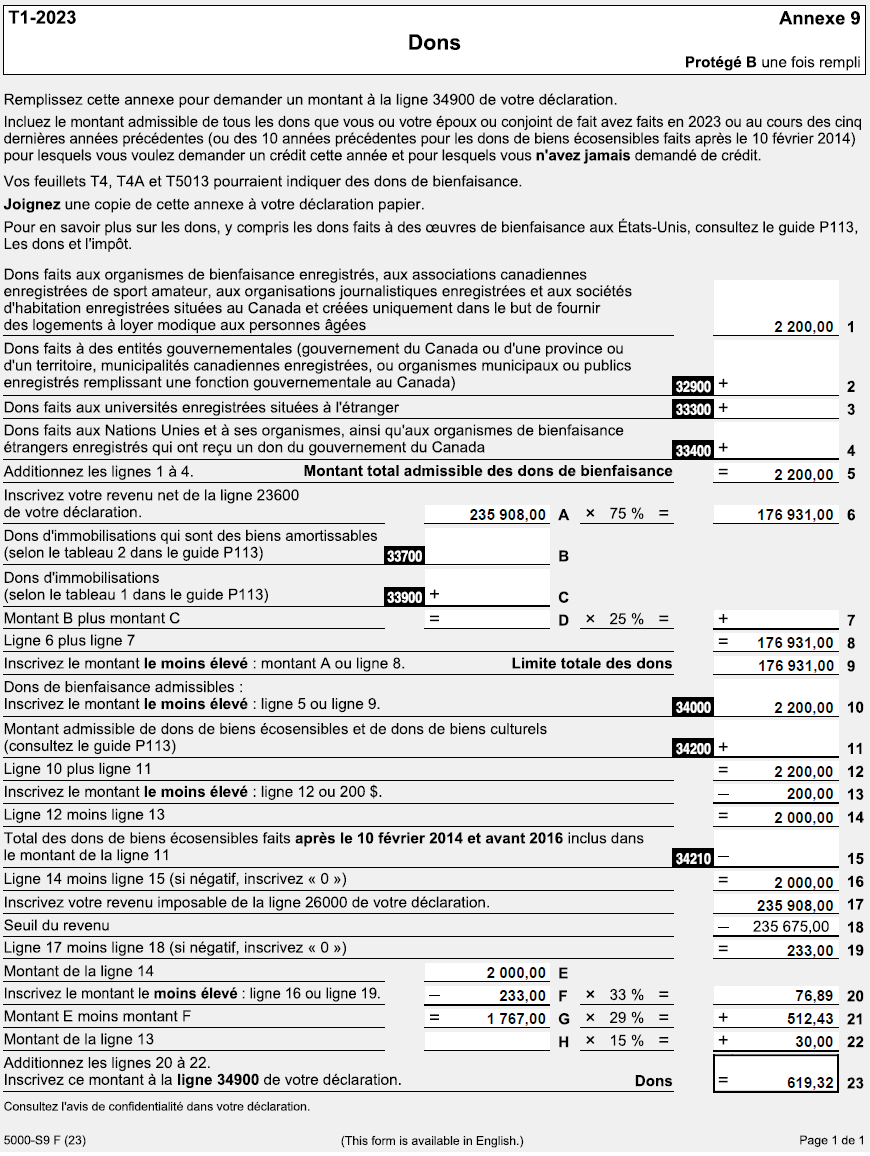
\includegraphics[width=.9\textwidth]{exercice/7-3/Q5/Annexe9.png}
	\caption[]{Exercice 3, annexe~9}
	\label{fig:chap7Exercice3Annexe9}
\end{figure}

\begin{sousQuestion}
	Sur quelle ligne de la déclaration T1 Jean réclame-t-il le crédit?
\end{sousQuestion}
À la ligne~34900 de sa T1.

\begin{sousQuestion}
	Jean devrait-il utiliser la grille 395 ou l'annexe~V pour calculer le montant de dons qui peut être réclamé sur sa TP-1 du Québec?
\end{sousQuestion}
Jean n'a aucun montant reporté des années précédentes et tous ses dons sont faits à des organismes de bienfaisance enregistrés, il peut donc utiliser la grille de calcul~395.

\begin{sousQuestion}
	Remplissez la \href{https://www.revenuquebec.ca/documents/fr/formulaires/tp/2023-12/TP-1.D.GR%282023-12%29.pdf}{grille de calcul~395}, présentée ci-dessous, en supposant que son revenu imposable au Québec est également de \numprint{235908}~\$.
\end{sousQuestion}
Grille de calcul pour ligne~395: figure~\ref{fig:chap7Exercice3Grille395}.
\begin{figure}
	\centering
	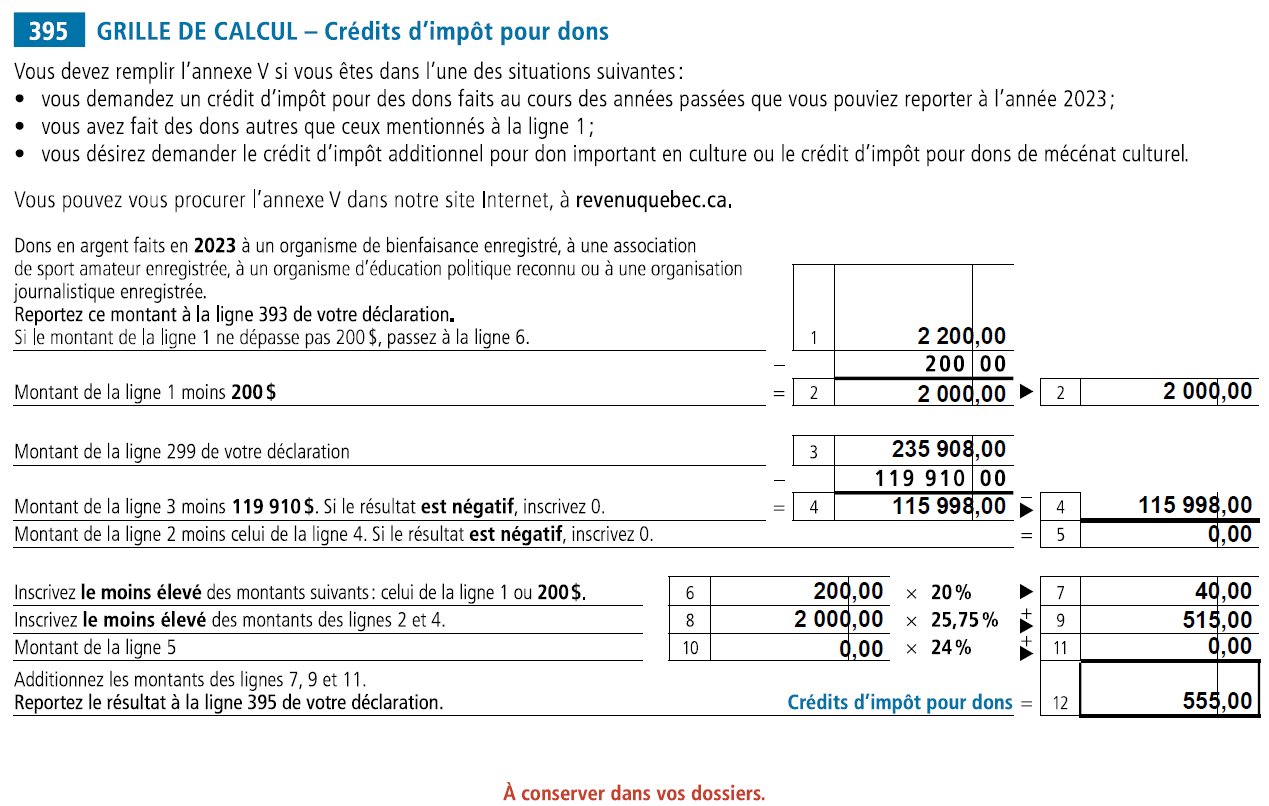
\includegraphics[width=.9\textwidth]{exercice/7-3/Q5/Grille395.png}
	\caption[]{Exercice 3, Grille 395}
	\label{fig:chap7Exercice3Grille395}
\end{figure}

\begin{question}
	Le montant inscrit à la ligne~299 de la déclaration TP1 de Jean Bérubé (Q5) est de \numprint{235908}~\$. Supposons qu'il ait reporté \numprint{1000}~\$ des années précédentes en plus des \numprint{2200}~\$ versés en 2023.
	
	Établissez le montant maximum au titre des dons de bienfaisance qu'il peut réclamer au Québec. Complétez l'\href{https://www.revenuquebec.ca/documents/fr/formulaires/tp/2023-12/TP-1.D.V%282023-12%29.pdf}{annexe~V}.
\end{question}
annexe~V, pages 1 à 3: figures~\ref{fig:chap7Exercice3AnnexeVp1}, \ref{fig:chap7Exercice3AnnexeVp2} et \ref{fig:chap7Exercice3AnnexeVp3}.

\begin{figure}
	\centering
	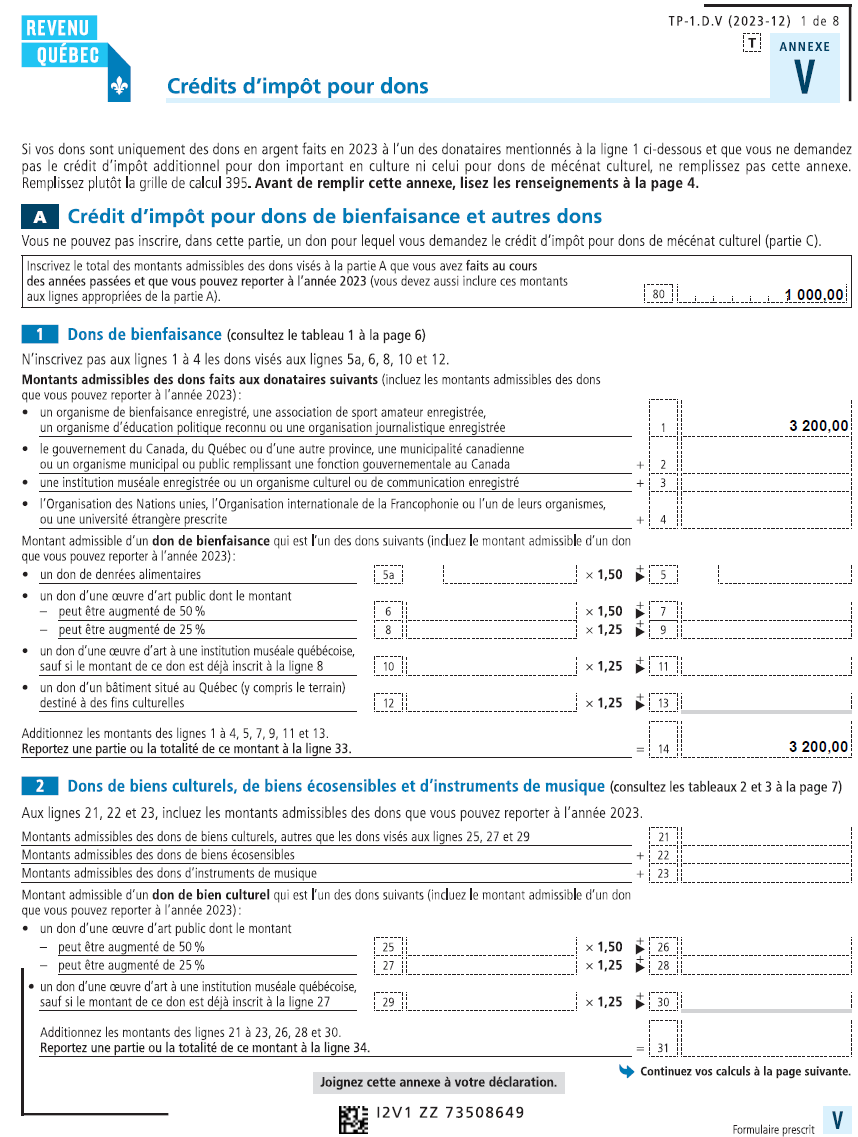
\includegraphics[width=.9\textwidth]{exercice/7-3/Q6/AnnexeVp1.png}
	\caption[]{Exercice 3, annexe~V page 1}
	\label{fig:chap7Exercice3AnnexeVp1}
\end{figure}
\begin{figure}
	\centering
	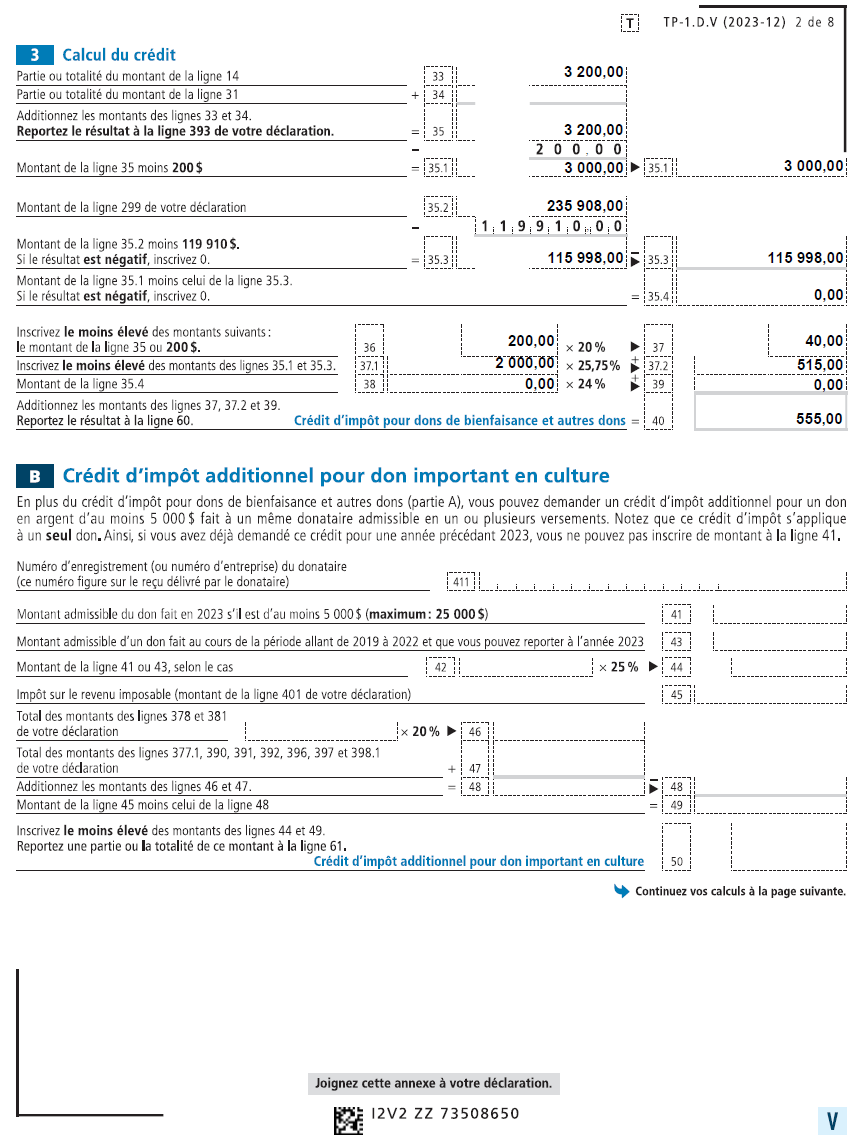
\includegraphics[width=.9\textwidth]{exercice/7-3/Q6/AnnexeVp2.png}
	\caption[]{Exercice 3, annexe~V page 2}
	\label{fig:chap7Exercice3AnnexeVp2}
\end{figure}
\begin{figure}
	\centering
	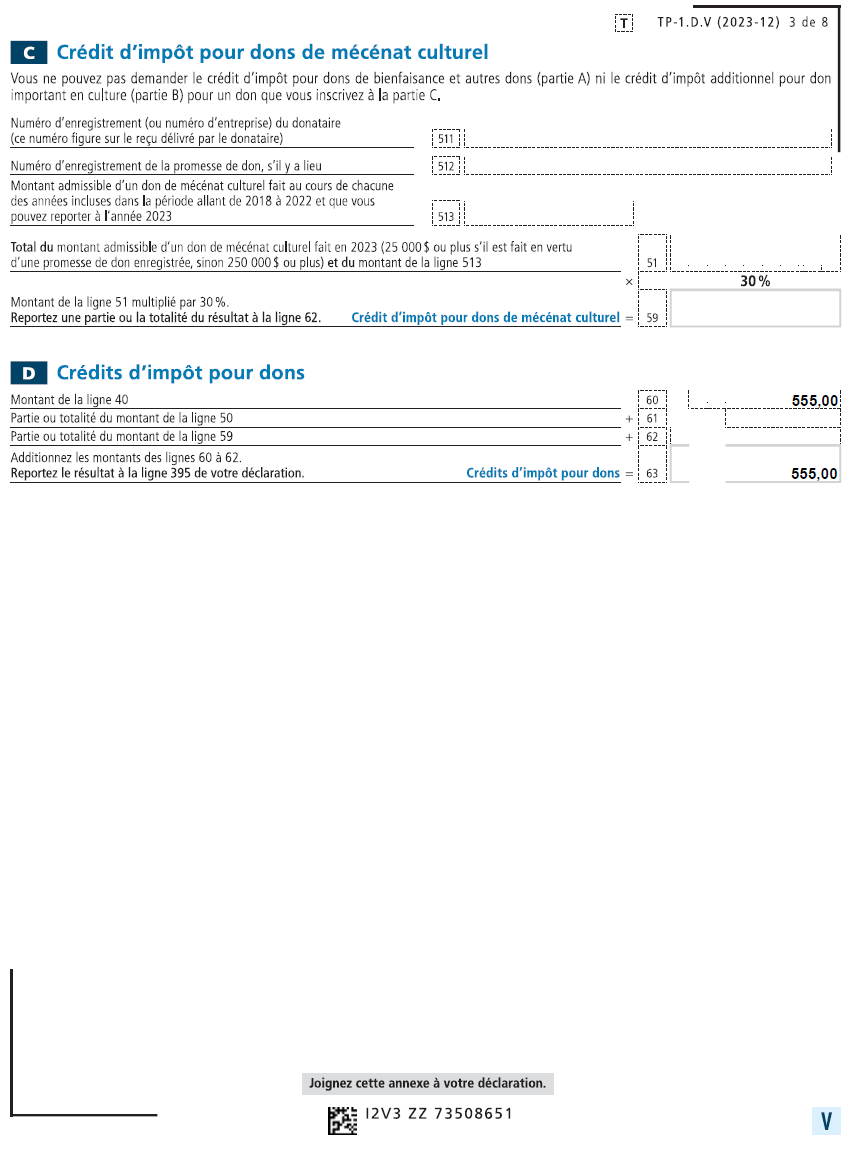
\includegraphics[width=.9\textwidth]{exercice/7-3/Q6/AnnexeVp3.png}
	\caption[]{Exercice 3, annexe~V page 3}
	\label{fig:chap7Exercice3AnnexeVp3}
\end{figure}

\begin{question}
	Bertrand et Catherine sont conjoints de fait depuis trois ans. En 2023, Bertrand a fait un don de bienfaisance de 175~\$ et Catherine, un de 150~\$. Le revenu net de Bertrand est de \numprint{28343}~\$ et celui de Catherine, de \numprint{16984}~\$.
	
	Au fédéral, établissez le crédit d'impôt pour chacun, selon ce qui serait le plus avantageux pour eux.
\end{question}
Au fédéral, il est à l'avantage du couple de faire une réclamation combinée afin de pouvoir bénéficier du crédit à un taux supérieur, plutôt qu'à un taux plus bas s'ils faisaient chacun une réclamation.
L'un ou l'autre des conjoints de fait peut faire cette réclamation combinée, en autant que leur impôt fédéral à payer n'a pas déjà été ramené à zéro.

Ainsi, le montant de la réclamation combinée pour l'année d'imposition est de:
\begin{itemize}
	\item Total des dons: 175~\$ + 150~\$ = 325~\$
	\item Le premier 200~\$ est à 15~\%, soit 30~\$
	\item Le total des dons restants est: 325~\$ $-$ 200~\$ = 125~\$
	\item Le restant des dons est à 29~\%, soit 36,25~\$
	\item Le total du crédit d'impôt des dons combinés: 66,25~\$
\end{itemize}

Séparément:
\begin{itemize}
	\item Le crédit d'impôt aurait été pour un: 175~\$ à 15~\% = 26,25~\$
	\item Le crédit d'impôt aurait été pour l'autre: 150~\$ à 15~\% = 22,50~\$
	\item En additionnant les crédit d'impôt, on arrive à 48,75~\$.
\end{itemize}

Une économie de 17,50~\$ en choisissant les dons combinés.

\begin{question}
	Michel Dubé, NAS 870 000 288, a droit au montant pour personne vivant seule. Il n'a aucune personne à charge. Le montant inscrit à la ligne~275 et à la ligne~299 de sa TP-1 est de \numprint{20000}~\$.
	
	Avant d'appliquer ses dons de bienfaisance, ses crédits d'impôt non remboursables sont de \numprint{2681,28}~\$, soit (\numprint{17183}~\$ $+$ \numprint{1969}~\$) $\times$ 14~\%. Michel a des reçus pour des dons de bienfaisance qui totalisent \numprint{1500}~\$. Il veut réclamer ces dons.
\end{question}
\setcounter{sousQuestion}{0}
\begin{sousQuestion}
	Quel montant pourrait-il réclamer au titre des dons de bienfaisance sur sa TP-1?
\end{sousQuestion}
Sur sa TP-1, Michel Dubé pourrait réclamer jusqu'à \numprint{1500}~\$, ce qui donne un crédit total de:
\[ 200~\$ \times 20~\% + \numprint{1300}~\$ \times 24~\% = 352~\$ \]

\begin{sousQuestion}
	Quelle partie du crédit d'impôt établi au point \og a \fg{}, a-t-il besoin pour réduire son impôt à payer à zéro? 
\end{sousQuestion}
Déterminons d'abord l'impôt à payer: \numprint{20000}~\$ de revenu imposable à 14~\% donne \numprint{2800}~\$ d'impôt à payer.

Les crédit d'impôt non remboursables sont les suivants:
\begin{itemize}
	\item Montant personnel de base: \numprint{17183}~\$
	\item Montant pour personne vivant seule: \numprint{1969}~\$
	\item Ces deux crédits à 14~\% donne \numprint{2681,28}~\$
\end{itemize}

Michel a donc besoin de 118,72~\$ (\numprint{2800}~\$ $-$ \numprint{2681,28}~\$) pour réduire son impôt à payer à zéro.

Déterminons le crédit d'impôt du don de \numprint{1500}~\$:
\begin{itemize}
	\item Les premiers 200~\$ à 20~\% donne 40,00~\$
	\item Le restant, c'est-à-dire \numprint{1300}~\$ est à 24~\%, ce qui donne: 312~\$.
\end{itemize}

Total du crédit d'impôt pour dons: 352~\$.

Il dispose donc d'un excédent de crédits disponibles de 233,28~\$ (352~\$ $-$ 118,72~\$).
\begin{itemize}
	\item Si Michel est célibataire, il peut reporter l'excédent, soit 972,00~\$ (233.28~\$/24~\%).
	\item Si Michel a une conjointe, il peut transférer le crédit excédentaire de 233,28~\$ à sa conjointe à la ligne~43
\end{itemize}



\section{Crédit d'impôt remboursable}
Les crédits d'impôt remboursables dont il est question dans le reste de ce chapitre ont des objectifs précis.

Les crédits d'impôt relatifs à la prime au travail (Québec) et l'allocation canadienne pour les travailleurs (fédéral) visent à encourager les contribuables à demeurer sur le marché du travail ou à l'intégrer.

Le crédit d'impôt pour mise aux normes d'installations d'assainissement des eaux usées résidentielles – Québec visant à aider les contribuables à mettre à niveau les anciens systèmes pour se conformer aux nouveaux règlements provinciaux.



\section{Allocation canadienne pour les travailleurs}
\begin{intro}
	L'\acrfull{act} s'adresse aux contribuables ou aux familles à faible revenu, qui ont gagné un revenu de travail ou un revenu de travail autonome. Les montants et les paramètres de niveau de revenu varient selon la province de résidence du bénéficiaire.
	
	L'ACT prend la forme d'un crédit d'impôt remboursable, qui peut être réclamée à la ligne~45300 de la déclaration T1, en utilisant l'annexe~6. Elle comprend un montant de base et un supplément pour les personnes handicapées. Le montant versé n'est pas imposable, tant au fédéral qu'au Québec.
\end{intro}

\subsection{Admissibilité}
Examiner la \og Liste de contrôle pour l'\acrfull{act} \fg{}, figures~\ref{fig:ACTp1} et \ref{fig:ACTp2}.
\begin{figure}
	\centering
	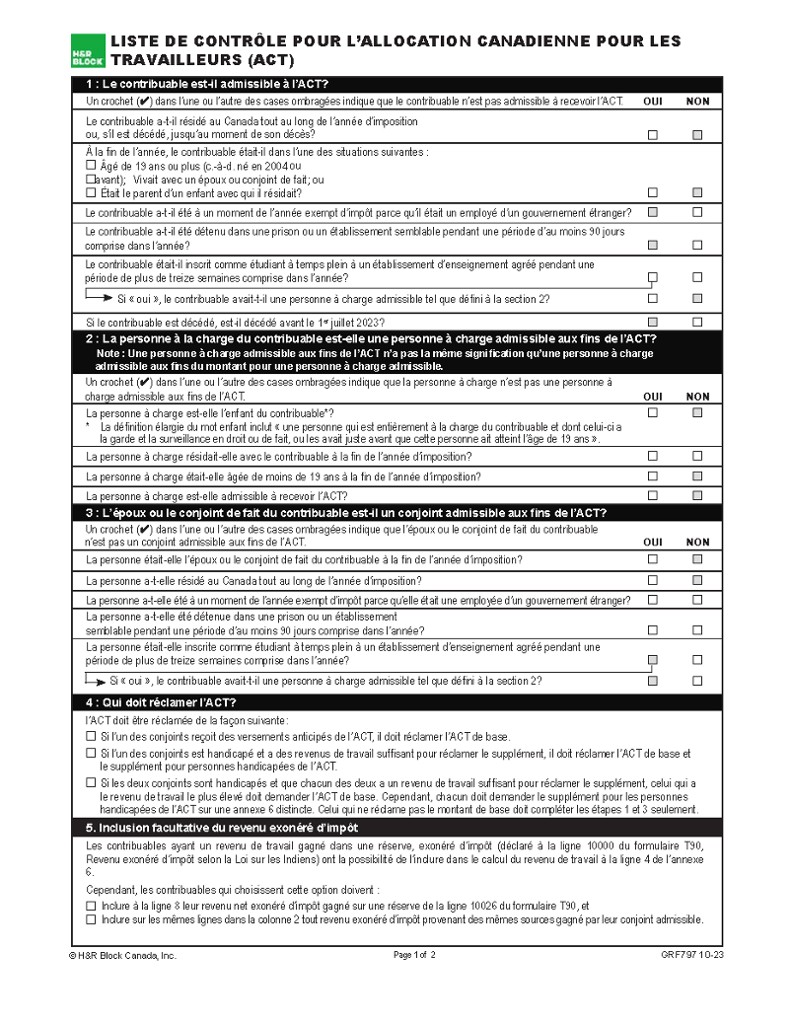
\includegraphics[width=.9\textwidth]{ACTp1.jpg}
	\caption{Liste de contrôle pour l'ACT, page 1}
	\label{fig:ACTp1}
\end{figure}
\begin{figure}
	\centering
	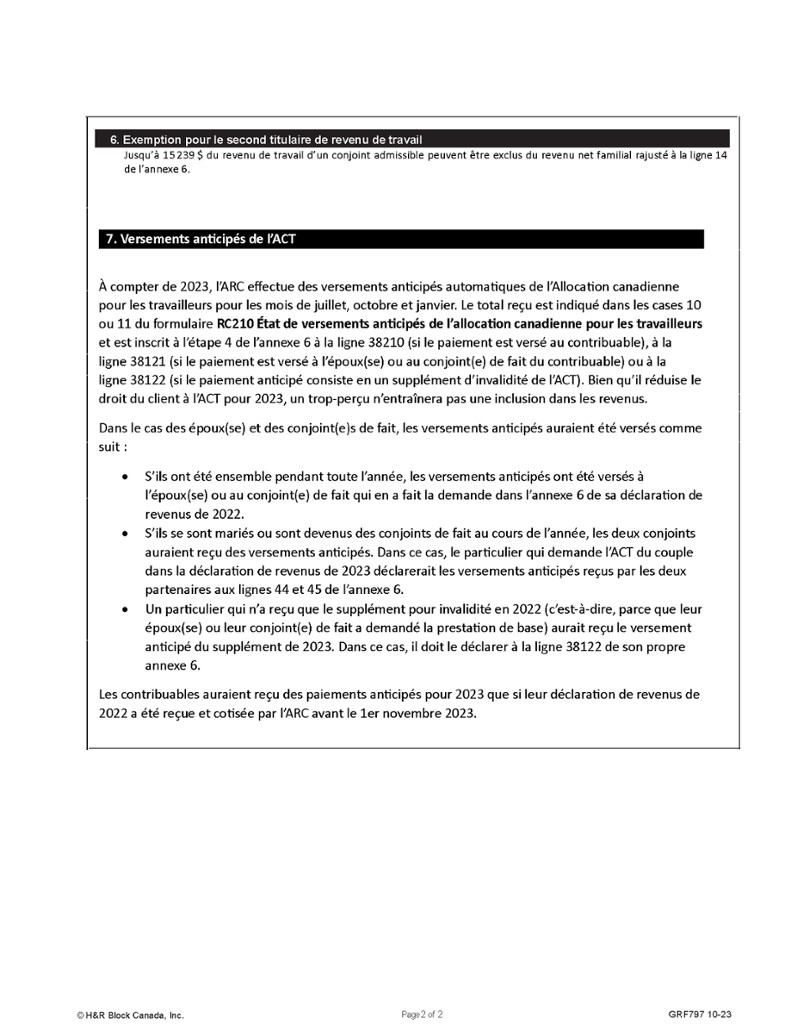
\includegraphics[width=.9\textwidth]{ACTp2.jpg}
	\caption{Liste de contrôle pour l'ACT, p. 2}
	\label{fig:ACTp2}
\end{figure}
Un contribuable peut demander l'ACT s'il satisfait à certaines conditions, notamment:
\begin{itemize}[label=\twemoji{check mark button}]
	\item Il était un résident du Canada durant toute l'année 2023;
	\item Il a gagné un revenu d'emploi ou d'entreprise;
	\item Il avait 19 ans ou plus le 31~décembre~2023. S'il avait moins de 19 ans, il résidait avec sa conjointe (épouse ou de fait) ou avec son enfant.
\end{itemize}

Un contribuable n'a pas droit à l'ACT si, en 2023:
\begin{itemize}[label=\twemoji{cross mark}]
	\item Il était inscrit comme étudiant à temps plein dans un établissement d'enseignement agréé* pour plus de 13 semaines durant l'année (sauf s'il avait une personne à charge admissible);
	\item Il a été détenu dans une prison ou dans un établissement semblable pour une période de 90 jours ou plus durant l'année; ou
	\item Il n'avait aucun impôt à payer au Canada parce qu'il était un agent ou un fonctionnaire d'un autre pays, par exemple, un diplomate.
\end{itemize}

\begin{note}
	Un établissement d'enseignement agréé inclut:
	\begin{itemize}[label=\twemoji{check box with check}]
		\item 	Les universités, collèges et autres institutions d'enseignement situés au Canada et offrant des cours de niveau postsecondaire;
		\item 	Les établissements d'enseignement reconnus par Emploi et développement social Canada et qui offrent des cours permettant d'acquérir ou d'améliorer des compétences professionnelles;
		\item 	Les universités situées à l'extérieur du Canada qui sont reconnues par l'ARC et où l'étudiant est inscrit dans un cours d'une durée d'au moins 13 semaines consécutives et menant à un diplôme; ou
		\item 	Les universités, collèges et autres institutions d'enseignement situés aux États-Unis offrant des cours de niveau postsecondaire si l'étudiant réside au Canada (près de la frontière) pendant toute l'année et fait la navette pour fréquenter l'école.
	\end{itemize}
\end{note}

\subsubsection{Conjoint admissible}
Aux fins de l'ACT, un conjoint admissible à la fin de 2023 est une personne qui:
\begin{itemize}[label=\twemoji{check mark button}]
	\item Est l'époux ou conjoint de fait du contribuable avec qui ce dernier vivait
	\item le 31~décembre~2023;
	\item Était un résident du Canada \textbf{pendant toute l'année} 2023;
	\item N'était pas inscrite comme étudiante à temps plein dans un établissement d'enseignement agréé pour plus de 13 semaines durant l'année, sauf si elle avait une personne à charge admissible à la fin de l'année;
	\item N'a pas été détenue dans une prison ou dans un établissement semblable pour une période de 90 jours ou plus durant l'année;
	\item N'était pas exempte de payer l'impôt sur le revenu du Canada pour la période durant laquelle elle était un agent, un fonctionnaire d'un autre pays, comme un diplomate, un membre de sa famille ou un de ses employés dans l'année.
\end{itemize}

\subsubsection{Personne à charge admissible}
Aux fins de l'ACT, une personne à charge admissible est une personne qui remplit toutes les conditions suivantes:
\begin{itemize}[label=\twemoji{check mark button}]
	\item Elle était l'enfant du contribuable ou celui de sa conjointe (épouse ou de fait);
	\item Elle était âgée de moins de 19 ans et résidait avec le contribuable au 31~décembre~2023;
	\item Elle n'était pas admissible à l'ACT pour 2023.
\end{itemize}
\begin{note}
	Il est important de ne pas confondre une \og personne à charge admissible \fg{} utilisée dans le calcul de l'ACT avec la définition utilisée dans le calcul du \og montant pour une personne à charge admissible\fg{} où le contribuable doit avoir été sans conjoint à un moment de l'année. Cette exigence ne s'applique pas ici.
\end{note}


\subsection{Calcul de l'ACT de base}
Le contribuable résidant au Québec doit remplir l'annexe~6 (spécifique au Québec) pour calculer le montant de l'ACT qui peut être réclamé à la ligne~45300 de sa déclaration T1.

La façon de remplir l'annexe~6 dépend des réponses du contribuable aux six questions de l'étape 1 qui exigent une réponse oui/non.

Contribuables , non admissibles au crédit d'impôt pour personnes handicapées (CIPH), doivent remplir les étapes 1 et 2.

Les contribuables admissibles au crédit du CIPH (discuté ci-dessous), doivent remplir les étapes 1 et 3.

Remplir l'étape 1 détermine deux montants:
\begin{itemize}
	\item Revenu de travail familial
	\item Revenu familial net rajusté
\end{itemize}

Le montant du revenu familial net rajusté doit être comparé aux seuils, selon la situation familiale du contribuable et son admissibilité au CIPH, au tableau de la page 3 de l'\href{https://www.canada.ca/fr/agence-revenu/services/formulaires-publications/trousses-impot-toutes-annees-imposition/trousse-generale-impot-prestations/quebec/5005-s6.html}{annexe~6}.

L'ACT ne peut être demandée que si le montant du revenu familial net rajusté est inférieur au seuil.

L'étape 2 de l'annexe~6 permet le calcul de l'ACT de base.

Le ou les contribuables doivent avoir un revenu de travail familial minimal pour demander l'ACT de base:
\begin{itemize}
	\item Comme contribuable célibataire, supérieur à \numprint{2400}~\$
	\item Avec un(e) conjoint(e) admissible, supérieur à \numprint{3600}~\$
	\item Si admissible au \acrshort{ciph}, supérieur à \numprint{1200}~\$
\end{itemize}

\begin{note}
	Les Indiens inscrits ayant un revenu exonéré d'impôt ont le choix d'inclure ou non le revenu exonéré d'impôt pour l'ACT. S'ils choisissent d'inclure leur revenu exonéré d'impôt à la ligne~4 de la partie~A, ils doivent également inclure le même montant à la ligne~8 de la partie~B.
\end{note}


\subsection{Supplément pour personnes handicapées de l'ACT}
Règle générale, un contribuable est reconnu comme une personne handicapée s'il a une déficience grave et prolongée des fonctions mentales ou physiques pendant au moins 12 mois consécutifs, ou s'il est prévu que la déficience aura cette durée.

Le contribuable qui a droit au montant pour personnes handicapées doit remplir l'étape 3 de l'annexe~6 pour demander le supplément pour personnes handicapées de l'ACT, et calculer le montant qui peut être réclamé à la ligne~45300 de sa T1. 


\subsection{Qui doit demander l'ACT?}
Les conditions suivantes s'appliquent pour demander l'Allocation canadienne pour les travailleurs:
\begin{itemize}
	\item Lorsqu'il y a un conjoint admissible, un seul des deux peut demander l'ACT de base;
	\item La personne qui a reçu les versements anticipés doit demander l'ACT de base;
	\item Si le contribuable a une personne à charge admissible, une seule personne peut demander l'ACT de base pour cette personne à charge;
	\item Si le contribuable avait un conjoint admissible et que l'un des deux a droit au montant pour personnes handicapées, cette personne (celle qui a droit au supplément) devrait demander l'ACT de base et le supplément;
	\item Si le contribuable avait un conjoint admissible et que tous les deux ont droit au montant pour personnes handicapées, un seul des deux peut demander l'ACT de base. Toutefois, chacun doit remplir une annexe~6 distincte afin de demander son supplément pour personnes handicapées de l'ACT.
\end{itemize}


\subsection{Paiements anticipés automatiques de l'Allocation canadienne pour les travailleurs}
À compter de 2023, l'ARC effectue désormais des paiements anticipés automatiques de l'Allocation canadienne pour les travailleurs en juillet, octobre~2023 et janvier~2024. Le total des trois paiements correspond à la moitié des droits du travailleur sur la déclaration de revenus 2022. Au cours des années précédentes, les contribuables avaient la possibilité de demander des paiements anticipés en remplissant le formulaire \href{https://www.canada.ca/fr/agence-revenu/services/prestations-enfants-familles/allocation-canadienne-travailleurs/rc210-etat-versements-anticipes-prestation-fiscale-revenu-travail.html}{RC210, État de l'\acrfull{aact}}. Cependant, il est désormais obligatoire.

Le total des paiements anticipés reçus est déclaré aux cases~10 ou 11 de \textbf{RC210, État de l'avance de l'allocation canadienne pour les travailleurs (AACT)} et est inscrit à l'étape 4 de l'annexe~6 sur le:
\begin{itemize}
	\item ligne~38120 si elle est payée au contribuable;
	\item ligne~38121, si elle est versée à l'époux ou conjoint de fait du contribuable;
	\item ligne~38122 si le paiement anticipé consistait en un supplément pour personnes handicapées de l'ACT.
\end{itemize}

Bien qu'il réduise le droit du client à l'ACT pour 2023, un paiement excédentaire n'entraînera pas d'inclusion dans le revenu C'est le cas même si le contribuable n'est pas admissible à l'ACT en 2023.



\section{La prime au travail}
\begin{intro}
	La prime au travail, accordée par le gouvernement du Québec, vise à encourager les travailleurs à faible et moyen revenu à entrer ou à demeurer sur le marché du travail. Il exige que les travailleurs aient gagné un revenu d'emploi au cours de l'année d'imposition.
\end{intro}
La prime au travail consiste en trois crédits d'impôt remboursables:
\begin{itemize}
	\item La prime au travail;
	\item La prime au travail adaptée;
	\item Le supplément à la prime au travail pour les anciens prestataires de l'aide sociale.
\end{itemize}
\begin{note}
	La prime au travail adaptée est offerte aux contribuables qui ont une déficience grave et prolongée des fonctions mentales ou physiques ou qui ont, dans l'année d'imposition en cours ou au cours de l'une des cinq années précédentes, en raison de contraintes sévères à l'emploi, des prestations du Programme de solidarité sociale.
\end{note}
Ils sont réclamés à la ligne~456 de la TP-1, en utilisant l'\href{https://www.revenuquebec.ca/documents/fr/formulaires/tp/2023-12/TP-1.D.P%282023-12%29.pdf}{annexe~P}. Le montant versé n'est pas imposable ni au fédéral ni au Québec. 


\subsection{Conditions de base}
Le contribuable peut réclamer les crédits d'impôt remboursables relatifs à la prime au travail (la prime au travail, la prime au travail adaptée et le supplément à la prime au travail pour le prestataire quittant l'assistance sociale), s'il remplit toutes les conditions de base suivantes:
\begin{itemize}
	\item Il résidait au Québec le 31~décembre~2023;
	\item Il est, selon le cas, un citoyen canadien, un Indien inscrit comme tel en vertu de la \textbf{Loi sur les Indiens}, un résident permanent au sens de la \textbf{Loi sur l'immigration et la protection des réfugiés} ou une personne à qui le Canada a accordé le droit d'asile en vertu de cette loi;
	\item Il est né avant le 1\ier{}~janvier~2006;
	\item S'il est né après le 31~décembre~2005:
	\begin{itemize}
		\item Ils avaient un(e) conjoint(e) au 31~décembre~2023;
		\item Ils étaient le parent d'un enfant qui résidait avec lui;
		\item Ils étaient reconnus comme mineur émancipé par une autorité compétente (par exemple, un tribunal);
	\end{itemize}
	\item Lui ou son conjoint au 31~décembre~2023, s'il y a lieu, déclare des revenus d'emploi, une subvention de recherche, des prestations du Programme de protection des salariés, ou des revenus d'une entreprise que lui ou sa conjointe exploite seuls ou comme associée y participant activement;
	\item Il n'a pas transféré à son père ou à sa mère un montant pour un enfant majeur aux études postsecondaires (ligne~20 de l'annexe~S);
	\item Personne n'a reçu à son égard le paiement d'allocation famille versé par Retraite Québec, sauf s'il a eu 18 ans avant le 1\ier{}~décembre~2023;
	\item Personne ne l'a inscrit comme enfant désigné, à la ligne~50 de l'annexe~P, pour demander le crédit relatif à la prime au travail;
	\item Il n' était pas étudiant à temps plein, sauf si, au 31~décembre~2023, il est le père ou la mère d'un enfant qui réside avec lui;
	\item Il n'était pas détenu en prison ou un établissement semblable le 31~décembre~2023 et, s'il y était détenu, n'y a pas passé plus de six mois en 2023.
\end{itemize}

\begin{note}
	Les résidents du Québec peuvent recevoir la Prime au travail à 18 ans et l'ACT à 19 ans.
\end{note}


\subsection{Calcul des crédits d'impôt relatifs à la prime au travail}
Utilisez l'\href{https://www.revenuquebec.ca/documents/fr/formulaires/tp/2023-12/TP-1.D.P%282023-12%29.pdf}{annexe~P} pour suivre la discussion ci-dessous.

\subsubsection{Revenu de travail (partie~A de l'annexe~P)}
La partie~A sert à déterminer les revenus de travail du contribuable et de son conjoint, s'il y a lieu.

Le revenu de travail d'un particulier et de son conjoint au 31~décembre aux fins du crédit d'impôt est constitué:
\begin{itemize}[label=\twemoji{check box with check}]
	\item De l'ensemble du revenu d'emploi inscrit aux lignes 101, 105 et 107;
	\item Du montant net des subventions de recherche inscrit à la ligne~154;
	\item Du revenu net d'entreprise reporté à l'annexe~L;
	\item Des prestations du Programme de protection des salariés que le particulier et sa conjointe ont inscrit à la ligne~154, avec le code \og 12 \fg{} à la case~153, de leur TP-1.
\end{itemize}

Le contribuable ne doit pas tenir compte des revenus d'emploi composés uniquement d'avantages imposables dont lui ou son conjoint au 31~décembre ont bénéficié en raison d'un ancien emploi. Ces revenus peuvent figurer à la case \og 211 \fg{} du relevé~1. Ils ne sont pas considérés comme un revenu de travail aux fins de l'annexe~P.

\subsubsection{Enfant à charge désigné (partie~B de l'annexe~P)}
Dans sa demande des crédits d'impôt relatifs à la prime au travail (prime au travail, prime au travail adaptée), le contribuable peut désigner un enfant comme personne à charge (partie~B de l'annexe~P). L'enfant doit être:
\begin{itemize}
	\item Soit un enfant pour lequel le contribuable ou sa conjointe au 31~décembre~2023 a reçu un paiement d'allocation famille de Retraite Québec; ou
	\item Soit un enfant né après le 31~décembre~2005 qui, en 2023, poursuivait à temps plein des études secondaires à la formation professionnelle ou des études postsecondaires, et pour lequel le contribuable ou sa conjointe a déduit (ou aurait pu déduire si cet enfant n'avait pas eu de revenu) un montant pour enfant mineur aux études postsecondaires à la ligne~21 de l'annexe~A; ou
	\item Soit un enfant né avant le 1\ier{}~janvier~2006, qui est son enfant ou celui de sa conjointe au 31~décembre et qui, en 2023, poursuivait à temps plein des études secondaires à la formation professionnelle ou des études postsecondaires pour lesquelles il a reçu un relevé~8 sur lequel il y a un montant à la case~A;
	\item Soit un enfant né après le 31~décembre~2005 qui résidait ordinairement avec le contribuable, qui n'est pas lui-même le parent d'un enfant avec lequel il réside, et qui n'est pas reconnu comme un mineur émancipé par une autorité compétente (par exemple, un tribunal);
	\begin{itemize}
		\item Si la garde de l'enfant est partagée en vertu d'un jugement ou d'une entente écrite, cet enfant est réputé résider ordinairement avec le contribuable, uniquement si le pourcentage du temps de garde qui lui est accordé, ou qui est accordé à son conjoint, pour l'année est d'au moins 40~\%.
	\end{itemize}
\end{itemize}

Le contribuable ne peut pas désigner un enfant comme personne à charge s'il était détenu en prison ou dans un établissement semblable le 31~décembre~2023 et s'il y était plus de six mois en 2023. 

\begin{note}
	L'enfant désigné perd le droit de demander, pour l'année, les crédits d'impôt relatifs à la prime au travail.
\end{note}

\subsubsection{Revenu familial (partie~C de l'annexe~P)}
Le revenu familial du contribuable correspond au montant de la ligne~275 de sa déclaration de plus, s'il y a lieu, le montant de la ligne~275 de la déclaration de sa conjointe au 31~décembre.

\subsubsection{Supplément à la prime au travail (partie D de l'annexe~P)}
Le supplément à la prime au travail est accordé aux prestataires qui quittent l'assistance sociale. Il s'agit d'un montant qui peut être accordé sur une base individuelle pour une période maximale de 12 mois consécutifs. Utiliser l'annexe~P et le relevé~5 pour suivre la discussion qui suit.

Le contribuable peut avoir droit à un supplément à la prime au travail et ainsi bénéficier d'un montant supplémentaire de 200~\$ par mois, s'il satisfait aux conditions d'admissibilité de base et à toutes les conditions additionnelles suivantes:
\begin{itemize}
	\item Le mois est compris dans une période de transition vers le travail.
	\item La \og période de transition vers le travail \fg{}:
	\begin{itemize}
		\item Commence le premier jour du mois où le contribuable cesse, en raison de ses revenus de travail ou de ceux de son conjoint à ce moment, soit de recevoir des prestations d'assistance sociale, soit de recevoir des prestations du programme Alternative jeunesse ou du Programme objectif emploi;
		\item Le premier mois de la période de transition vers le travail est indiqué à la case~T du relevé~5; et se termine au plus tard le dernier jour du 11e mois qui suit ce mois, ou le dernier jour du mois qui précède le mois pour lequel le contribuable redevient admissible à l'assistance sociale. Le mois du retour à une aide financière de dernier recours ou une aide financière du programme Alternative jeunesse ou du Programme objectif emploi est indiqué à la case~U du relevé~5;
	\end{itemize}
	\item Il a reçu de l'aide financière de l'assistance sociale ou de l'aide financière du programme Alternative jeunesse ou du Programme objectif emploi pendant au moins 24 mois des 30 mois précédant immédiatement le début de la période de transition vers le travail. La mention \og Oui \fg{} ou
	\item \og Non \fg{} dans la case~R du relevé~5 indique si le contribuable a reçu ou non une aide;
	\item Pour le premier mois de la période de transition vers le travail, il détenait un carnet de réclamation délivré par le ministère de l'Emploi et de la Solidarité sociale lui permettant de bénéficier de certains services dentaires et pharmaceutique, sauf s'il recevait des prestations du programme Alternative jeunesse ou du Programme objectif emploi pour le mois qui précède le début de sa période de transition vers le travail. La mention \og Oui \fg{} ou \og Non \fg{} dans la case~S du relevé~5 indique si le contribuable détenait ou non un carnet de réclamation;
	\item Il a un revenu de travail d'au moins 200~\$ durant le mois pour lequel il demande le supplément.
\end{itemize}

Le nombre de mois compris dans l'année et dans la période de transition vers le travail pendant lesquels le contribuable n'a pas reçu une aide financière de dernier recours figure à la case~V du relevé~5. Il doit être inscrit à la ligne~57 de l'annexe~P. Lui et sa conjointe doivent produire chacun une annexe~P distincte s'ils ont reçu tous les deux un relevé~5 sur lequel un nombre de mois est inscrit à la case \og V \fg{}.

Le \og nombre de mois pour lesquels le contribuable remplit les conditions d'admissibilité \fg{} correspond à la période comprise entre le début de la période de transition pour le travail (case~T) et son retour à l'aide financière (case~U). Ce nombre doit être inscrit à la ligne~58 de l'annexe~P.

Se rappeler que le supplément à la prime au travail est de 200~\$ par mois et qu'il peut être accordé pour une période maximale de 12 mois consécutifs. Par conséquent, pour une période de travail continue d'au moins 12 mois, il peut atteindre \numprint{2400}~\$ pour une personne seule et, dans le cas d'un couple, \numprint{4800}~\$ si chacun des conjoints a intégré le marché du travail.

\subsubsection{Prime au travail (partie E de l'annexe~P, colonne 1)}
Le contribuable a droit à une prime au travail s'il remplit les conditions suivantes:
\begin{itemize}[label=\twemoji{check mark button}]
	\item Il a un conjoint au 31~décembre et son revenu de travail (ligne~29 plus ligne~49 de l'annexe~P) dépasse \numprint{3600}~\$. La section \og Particulier avec conjoint \fg{} de la partie E doit être remplie; ou
	\item Il n'a pas de conjoint au 31~décembre (une personne seule ou une famille monoparentale) et son revenu de travail (ligne~29 de l'annexe~P) dépasse \numprint{2400}~\$. La section \og Particulier sans conjoint \fg{} de la partie E doit être remplie;
	\item Son revenu familial est inférieur au revenu familial maximal qui s'applique à lui en fonction de sa situation familiale et de son revenu de travail.
\end{itemize}

\subsubsection{Prime au travail adaptée (partie E de l'annexe~P, colonne 2)}
Comme indiqué à la partie E de l'annexe~P, le contribuable qui veut réclamer la prime au travail adaptée doit tout d'abord remplir la colonne 1, \textbf{Prime au travail}, afin de calculer la prime au travail qu'il pourrait réclamer. Par la suite, il doit remplir la colonne 2, \textbf{Prime au travail adaptée}, si lui ou sa conjointe, au 31~décembre:
\begin{itemize}
	\item Ont reçu en 2023, au cours de l'année ou au cours de l'une des cinq années précédentes, en raison de contraintes sévères à l'emploi, des prestations du Programme de solidarité sociale ou une allocation pour contraintes sévères à l'emploi;
	\item Avaient droit, en 2023, au montant pour déficience grave et prolongée des fonctions mentales ou physiques.
\end{itemize}

Le contribuable a droit à une prime au travail adaptée s'il remplit toutes les conditions de base énumérées précédemment à la rubrique \og Prime au travail \fg{}, plus l'une ou l'autre des conditions additionnelles présentées ci-dessus. Si le contribuable est admissible à la prime au travail adaptée, il peut réclamer à la ligne~456 de sa déclaration~TP-1 \textbf{le montant le plus élevé} entre la prime au travail (ligne~84 de la colonne 1) et la prime au travail adaptée (ligne~84 de la colonne 2).

Le contribuable n'a pas droit à la prime au travail adaptée si son revenu de travail (ligne~29 de l'annexe~P, s'il n'avait pas de conjointe au 31~décembre, ou le total des lignes~29 et 49, s'il avait une conjointe au 31~décembre) ne dépasse pas \numprint{1200}~\$.


\subsection{Versements anticipés des crédits d'impôt relatifs à la prime au travail}
La prime au travail et la prime au travail adaptée peuvent être versées à l'avance (versements anticipés mensuels), plutôt que d'être demandées lors de la production annuelle de la déclaration de revenus provinciale.

Pour recevoir les versements anticipés en 2023, le contribuable doit fournir une estimation de son revenu de travail de 2023 en remplissant le formulaire \href{https://www.revenuquebec.ca/documents/fr/formulaires/tpz/TPZ-1029.8.P(2023-10).pdf}{TPZ-1029.8. P, Crédit d'impôt pour prime au travail – Demande de versements anticipés}, disponible dans un des bureaux de Revenu Québec. Si le contribuable a une conjointe qui estime avoir droit à la prime au travail ou à la prime au travail adaptée, un seul des deux peut faire une demande de versements anticipés pour le couple.

\subsubsection{Traitement fiscal des paiements anticipés sur Relevé~19}
En 2023, si un contribuable a reçu des versements anticipés pour la prime au travail, la prime au travail adaptée ou le supplément à la prime au travail (pour les personnes qui ont cessé de recevoir l'aide sociale), il recevra un Relevé~19.

Il doit inscrire le montant de la case~A et/ou de la case~B du relevé~19 à la ligne~441 de sa TP-1.

Le contribuable qui a reçu des versements anticipés de la prime au travail ou le supplément à la prime au travail doit remplir l'annexe~P pour calculer le montant exact des crédits d'impôt remboursables de la prime au travail auxquels il a droit en raison de ses revenus de 2023.

Toute différence entre le montant calculé et les versements anticipés affectera le remboursement ou le solde dû du contribuable.

\subsection{Partage du crédit d'impôt relatif à la prime au travail}
Il est possible pour chaque conjoint d'un couple de partager les crédits d'impôt de la prime au travail. Pour ce faire, chaque conjoint doit remplir sa propre annexe~P, puis indiquer le montant du crédit que son conjoint demande à la ligne~86.

\rqg[s]{73 à 76}



\section{Bouclier fiscal}
\begin{intro}
	Le contribuable qui reçoit un crédit d'impôt de prime au travail ou de frais de garde d'enfants peut voir ces crédits d'impôts diminuer si ses revenus de travail augmentent.
	
	Dans cette situation, le contribuable peut réclamer le crédit d'impôt remboursable \og Bouclier fiscal \fg{} qui vise à compenser une partie de ces pertes.
\end{intro}
Pour calculer ce crédit, le contribuable doit tenir compte de sa situation familiale et son revenu ainsi que de celui de sa conjointe au 31~décembre~2023.

Ce crédit est calculé pour une hausse maximale de revenu de travail de \numprint{4000}~\$ par conjoint.


\subsection{Détermination du crédit}
Le contribuable qui a résidé au Québec le 31~décembre~2023 et que lui ou sa conjointe a droit aux crédits d'impôt relatifs à la prime au travail ou au crédit d'impôt pour frais de garde d'enfants, il peut demander un crédit d'impôt Bouclier fiscal s'il est dans l'une des situations suivantes:
\begin{itemize}
	\item Il n'a pas de conjointe au 31~décembre~2023:
	\begin{itemize}
		\item Son revenu net, inscrit à la ligne~275 de votre déclaration de revenus de 2023, est plus élevé que celui inscrit dans votre déclaration de revenus de 2022,
		\item Son revenu de travail admissible, établi selon leur déclaration de revenus de 2023, est plus élevé que celui établi selon la déclaration de revenus de 2022;
	\end{itemize}
	\item Il a une conjointe au 31~décembre~2023:
	\begin{itemize}
		\item Son revenu familial net (montant de la ligne~275 de votre déclaration plus celui de la ligne~275 de la déclaration du conjoint) de l'année 2023 est plus élevé que celui de l'année 2022,
		\item Son revenu de travail admissible ou celui du conjoint, établi selon la déclaration de revenus de 2023, est plus élevé que celui établi selon la déclaration de revenus de 2022.
	\end{itemize}
\end{itemize}

Le mécanisme du bouclier fiscal consiste à calculer un revenu familial modifié (réduit). La réduction correspond à 75~\% du moindre des montants suivants:
\begin{itemize}
	\item L'augmentation du revenu familial net en 2023 par rapport à 2022;
	\item L'augmentation du revenu de travail admissible ou du revenu de travail admissible conjoint en 2023 par rapport à 2022.
\end{itemize}

\begin{note}
	L'augmentation admissible du revenu d'emploi est plafonnée à \numprint{4000}~\$ pour chaque conjoint. Par conséquent, la réduction maximale pour un contribuable célibataire est de \numprint{3000}~\$, et pour un couple, elle est de \numprint{6000}~\$.
\end{note}

\subsection{Demander le crédit d'impôt Bouclier fiscal}
Le contribuable doit cocher la case~5 de l'annexe~P ou la case~99 de l'annexe~C pour réclamer le \og Bouclier fiscal \fg{}. Revenu Québec déterminera le montant du crédit qu'il aura droit. Le contribuable qui désire calculer le montant du crédit d'impôt lui-même, il doit utiliser le formulaire \href{https://www.revenuquebec.ca/fr/services-en-ligne/formulaires-et-publications/details-courant/tp-1029-bf/}{TP-1029.BF -- Crédit d'impôt Bouclier fiscal}.

Le crédit accordé pour le Bouclier fiscal est d'un maximum de 300~\$ pour un contribuable célibataire et d'un maximum de 600~\$ pour un couple. Tout montant pour frais de garde d'enfants sera ajouté à ce montant, si admissible.

Le crédit d'impôt Bouclier fiscal peut être réclamé par l'un ou l'autre des conjoints, ou partagé entre eux.



\section{Mise aux normes d'installations d'assainissement des eaux usées résidentielles -- Québec}
\begin{intro}
	C'est un crédit d'impôt remboursable qui est offert au contribuable qui a payé, après le 31~mars~2017, une dépense pour faire exécuter des travaux de mise aux normes des installations d'assainissement des eaux usées à l'égard de son lieu principal de résidence ou son chalet habitable à l'année. 
\end{intro}
Ces travaux doivent être exécutés en vertu d'une entente conclue après le 31~mars~2017 et avant le 1\ier{}~avril~2027.

Ce crédit est égal à 20~\% de la partie des dépenses admissibles payées pour ces travaux qui dépassent \numprint{2500}~\$, jusqu'à concurrence d'un crédit d'impôt maximal de \numprint{5500}~\$ par habitation admissible.


\subsection{Détermination du crédit}
Pour demander le crédit d'impôt pour mise aux normes d'installations d'assainissement des eaux usées résidentielles si toutes les conditions suivantes sont remplies:
\begin{itemize}[label=\twemoji{check mark button}]
	\item Est résident au Québec le 31~décembre~2023 ou, si a cessé de résider au Canada au cours de 2023, a résidiez au Québec le jour où a cessé de résider au Canada.
	\item Le contribuable ou son conjoint a conclu un contrat avec un entrepreneur qualifié après le 31~mars~2017 pour améliorer le système de traitement des eaux usées résidentielles d'un logement admissible.
	\item Demander le crédit d'impôt pour les dépenses admissibles payées en 2023.
\end{itemize}

Si un contribuable a déjà engagé et déduit des dépenses admissibles entre
le 1\ier{}~avril~2017 et le 31~décembre~2022 dans des déclarations de revenus antérieures, il n'est pas tenu de réduire son montant de \numprint{2500}~\$ pour les dépenses admissibles engagées en 2023. Le montant cumulatif maximal de \numprint{5500}~\$ doit toujours être respecté.


\subsection{Habitation admissible}
Pour être admissible, l'habitation doit remplir les conditions suivantes:
\begin{itemize}[label=\twemoji{check mark button}]
	\item Elle est située au Québec. 
	\item Sa construction a été complétée avant le 1\ier{}~janvier~2017. 
	\item Elle ne fait pas l'objet d'un avis d'expropriation, d'un avis d'intention d'exproprier, d'une réserve pour fins publiques, d'un préavis d'exercice d'un droit hypothécaire inscrit au bureau de la publicité des droits ou de toute autre procédure remettant en cause le droit de propriété. 
	\item Elle est une résidence isolée au sens du Règlement sur l'évacuation et le traitement des eaux usées des résidences isolées4, ou fait partie d'une telle résidence, et est visée par le champ d'application de l'article~2 de ce règlement. 
	\item Elle est votre lieu principal de résidence au moment où les dépenses ont été engagées. Dans le cas d'un chalet, celui-ci doit être habitable à l'année et normalement occupé par vous-même.
\end{itemize}


\subsection{Entente de service}
Les travaux reconnus à l'égard de l'habitation admissible doivent être effectués conformément à une entente conclue après le 31~mars~2017 et avant le 1\ier{}~avril~2027 entre un entrepreneur et l'une des personnes suivantes: 
\begin{itemize}[label=\twemoji{check mark button}]
	\item contribuable
	\item conjoint ou conjointe du contribuable au moment de la conclusion de l'entente; 
	\item toute autre personne qui est copropriétaire ou le conjoint ou la conjointe de cette autre personne au moment de la conclusion de l'entente. 
\end{itemize}

Si l'habitation admissible est située dans un immeuble en copropriété (condominium), l'entente doit avoir été conclue par le syndicat des copropriétaires de l'immeuble.

\subsection{Entrepreneur}
Les travaux doivent être effectués par un entrepreneur:
\begin{itemize}[label=\twemoji{check mark button}]
	\item qui n'est ni propriétaire ou copropriétaire de l'habitation ni le conjoint ou la conjointe du ou de la propriétaire, ou d'un ou d'une copropriétaire, au moment de la conclusion de l'entente; 
	\item qui a un établissement au Québec au moment de la conclusion de l'entente; 
	\item qui est titulaire, au moment de la réalisation des travaux, d'une licence de la sous-catégorie~2.4, \og Entrepreneur en systèmes d'assainissement autonome \fg{}, délivrée par la Régie du bâtiment du Québec et qui a obtenu le cautionnement de licence.
\end{itemize}


\subsection{Travaux de mise aux normes des installations d'assainissement des eaux usées}
Les travaux reconnus pour les fins de ce crédit sont ceux qui portent sur la construction, la rénovation, la modification, la reconstruction, le déplacement ou l'agrandissement d'une installation d'évacuation, de réception ou de traitement des eaux usées, des eaux de cabinet d'aisances ou des eaux ménagères d'une habitation admissible.


\subsection{Dépenses admissibles}
Les dépenses admissibles devront être payées dans l'année et correspondront au:
\begin{itemize}[label=\twemoji{check mark button}]
	\item Coût des permis nécessaires à la réalisation des travaux, y compris le coût des études réalisées pour obtenir de tels permis;
	\item Coût (taxes incluses) des biens:
	\begin{itemize}
		\item qui ont servi à la réalisation des travaux,
		\item qui ont été fournis par l'entrepreneur ou achetés chez un commerçant inscrit au fichier de la TVQ, après le 31~mars~2017;
	\end{itemize}
	\item Coût (taxes incluses) des services fournis par l'entrepreneur pour la réalisation des travaux;
	\item Coût des travaux nécessaires à la remise en état des lieux.
	\item 
\end{itemize}


\subsection{Dépenses non admissibles}
Les dépenses non admissibles comprennent:
\begin{itemize}[label=\twemoji{check mark button}]
	\item Les dépenses se rapportant à une partie de l'habitation utilisée pour gagner des revenus d'entreprise ou de location;
	\item Les dépenses qui servent à financer le coût des travaux;
	\item Les dépenses attribuables à des biens ou à des services fournis par une personne ayant un lien de dépendance avec vous ou avec l'un des autres propriétaires de l'habitation, sauf si cette personne est inscrite au fichier de la TVQ.
\end{itemize}


\subsection{Demande du crédit}
Pour bénéficier du crédit d'impôt pour mise aux normes d'installations d'assainissement des eaux usées résidentielles, un particulier doit joindre à sa déclaration de revenus le formulaire \href{https://www.revenuquebec.ca/documents/fr/formulaires/tp/TP-1029.AE(2022-10).pdf}{TP-1029.AE -- Crédit d'impôt pour mise aux normes d'installations d'assainissement des eaux usées résidentielles}.

Ce formulaire contient la description des travaux réalisés, leur coût, des renseignements sur l'habitation qui a fait l'objet des travaux et des renseignements sur les entrepreneurs ayant réalisé les travaux.

De plus, l'entrepreneur responsable des travaux doit attester que les biens et les services répondent à des normes reconnues. Pour ce faire, il doit remplir et signer le formulaire \href{https://www.revenuquebec.ca/documents/fr/formulaires/tp/TP-1029.AE.A(2023-10).pdf}{TP-1029.AE.A -- Attestation de conformité de biens aux normes d'installations d'assainissement des eaux usées résidentielles} et le remettre à son client. Ce formulaire atteste que les biens et les services se rapportent à des travaux des installations d'assainissement des eaux usées résidentielles.

Le crédit d'impôt est demandé à la ligne~462, avec le code 33 à la case~461, de la TP-1.



\section{Exercice 4}
\setcounter{question}{0}
\begin{question}
	Maxime a 19 ans. Il poursuit des études postsecondaires à temps plein. Un montant de \numprint{7074}~\$ apparaît à la case~A de son Relevé~8. Maxime a travaillé durant l'été et a gagné \numprint{3800}~\$. Le montant inscrit à la ligne~275 de sa déclaration~TP-1 est de \numprint{3572}~\$.
	
	Au Québec, Maxime peut-il réclamer les crédits d'impôt relatifs à la prime au travail? Expliquez votre réponse.
\end{question}
Depuis 2015, les étudiants postsecondaires à temps plein ne sont plus admissibles à la prime au travail à moins qu'ils ne soient le père ou la mère d'un enfant qui habite avec eux. Ainsi, Maxime n'est pas en mesure de réclamer la prime.

\begin{question}
	Marguerite Bégin a reçu un Relevé~19, cf. figure~\ref{fig:chap7Exercice4RL19}.
	\begin{figure}
		\centering
		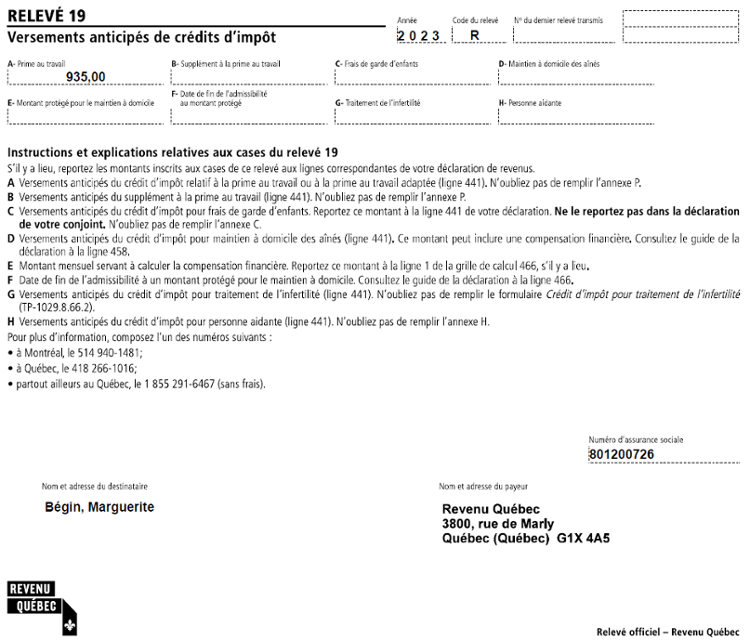
\includegraphics[width=.9\textwidth]{exercice/7-4/Q2/RL19.png}
		\caption[]{Exercice 4, Relevé~19}
		\label{fig:chap7Exercice4RL19}
	\end{figure}
\end{question}
\setcounter{sousQuestion}{0}
\begin{sousQuestion}
	Que doit-elle faire du montant inscrit à la case~A de son relevé~19?
\end{sousQuestion}
Marguerite doit déclarer le montant de la case~A de son Relevé~19 à la ligne~441 de sa déclaration TP1.

\begin{sousQuestion}
	Doit-elle remplir l'annexe~P? Expliquez votre réponse.
\end{sousQuestion}
Oui. Elle doit remplir l'annexe~P.

Puisque Marguerite doit déclarer ses versements anticipés à la ligne~441 de sa TP1, et augmente donc ses impôts provinciaux à payer, elle devrait remplir l'annexe~P pour compenser le montant qu'elle doit déclarer à la ligne~441. Elle pourra alors réclamer le crédit d'impôt auquel elle a droit à la ligne~456 de sa déclaration TP1, éliminant ainsi en tout ou en partie les versements anticipés qu'elle a reçus.

\begin{sousQuestion}
	Le crédit qu'elle pourrait réclamer en remplissant l'annexe~P est-il imposable sur les déclarations fédérale et du Québec? Expliquez votre réponse.
\end{sousQuestion}
Non. Il s'agit d'un crédit d'impôt remboursable non imposable tant au fédéral qu'au Québec.

\begin{question}
	Depuis trois ans, Robert Lanier reçoit de l'assistance sociale. Le 1\ier{}~juillet~2023, il a quitté l'assistance sociale pour occuper un emploi durant cinq mois. Il a gagné \numprint{9600}~\$. Il est retourné sur l'assistance sociale le 2~décembre~2023. Il a reçu le relevé~5 de la 
	figure~\ref{fig:chap7Exercice4RL5}.
	\begin{figure}
		\centering
		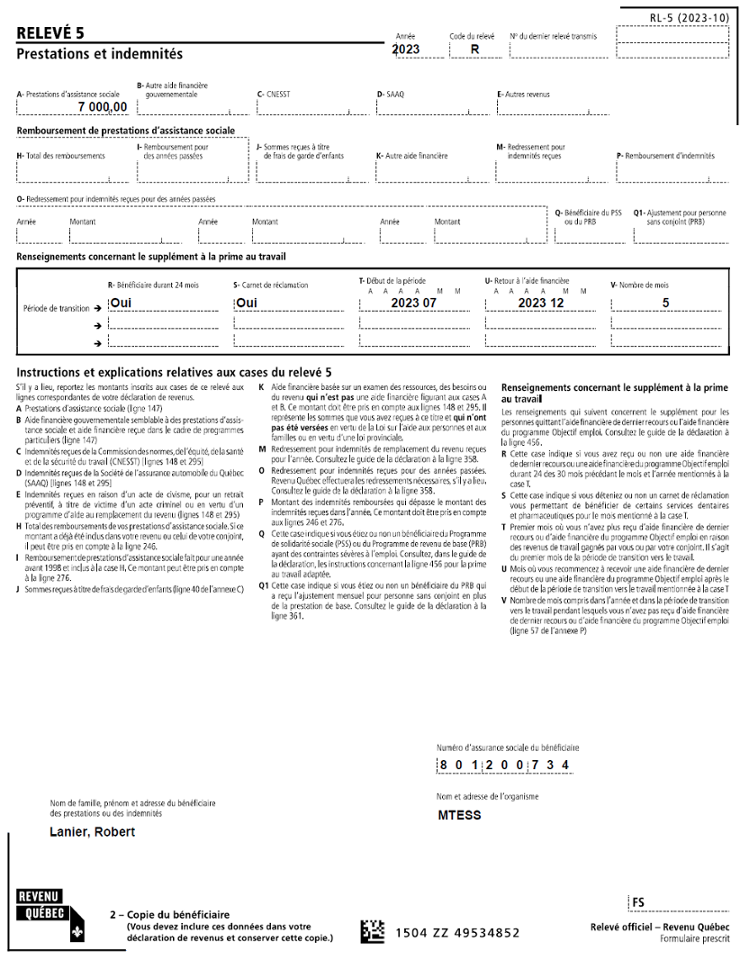
\includegraphics[width=.9\textwidth]{exercice/7-4/Q3/RL5.png}
		\caption[]{Exercice 4, Relevé~5}
		\label{fig:chap7Exercice4RL5}
	\end{figure}
\end{question}
\setcounter{sousQuestion}{0}
\begin{sousQuestion}
	Robert est-il admissible au supplément à la prime au travail payée par le Québec? Expliquez votre réponse.
\end{sousQuestion}
Oui. Il répond aux critères d'admissibilité de base: il a reçu de l'aide sociale pendant plus de 24 des 30 derniers mois précédant le mois au cours duquel il a cessé de la recevoir pour entrer en emploi.

\begin{sousQuestion}
	Si Robert Lanier peut réclamer le supplément à la prime au travail, compléter l'\href{https://www.revenuquebec.ca/documents/fr/formulaires/tp/2023-12/TP-1.D.P%282023-12%29.pdf}{annexe~P}. Par la suite, réclamer le montant à la ligne appropriée de la page 4 de sa TP-1.
	Notez que le montant de la ligne~248 de sa TP-1 (Bonification au RRQ) est de 61,00~\$.
\end{sousQuestion}
Le montant de la ligne~52 de l'annexe~P, figure~\ref{fig:chap7Exercice4AnnexePp1}, résultant du calcul suivant:
\begin{center}
	\numprint{9600}~\$ + \numprint{7000}~\$ $-$ 576~\$ (déduction du travailleur) $-$ 61~\$ (RRQ prime) = \numprint{15963}~\$
\end{center}
\begin{figure}
	\centering
	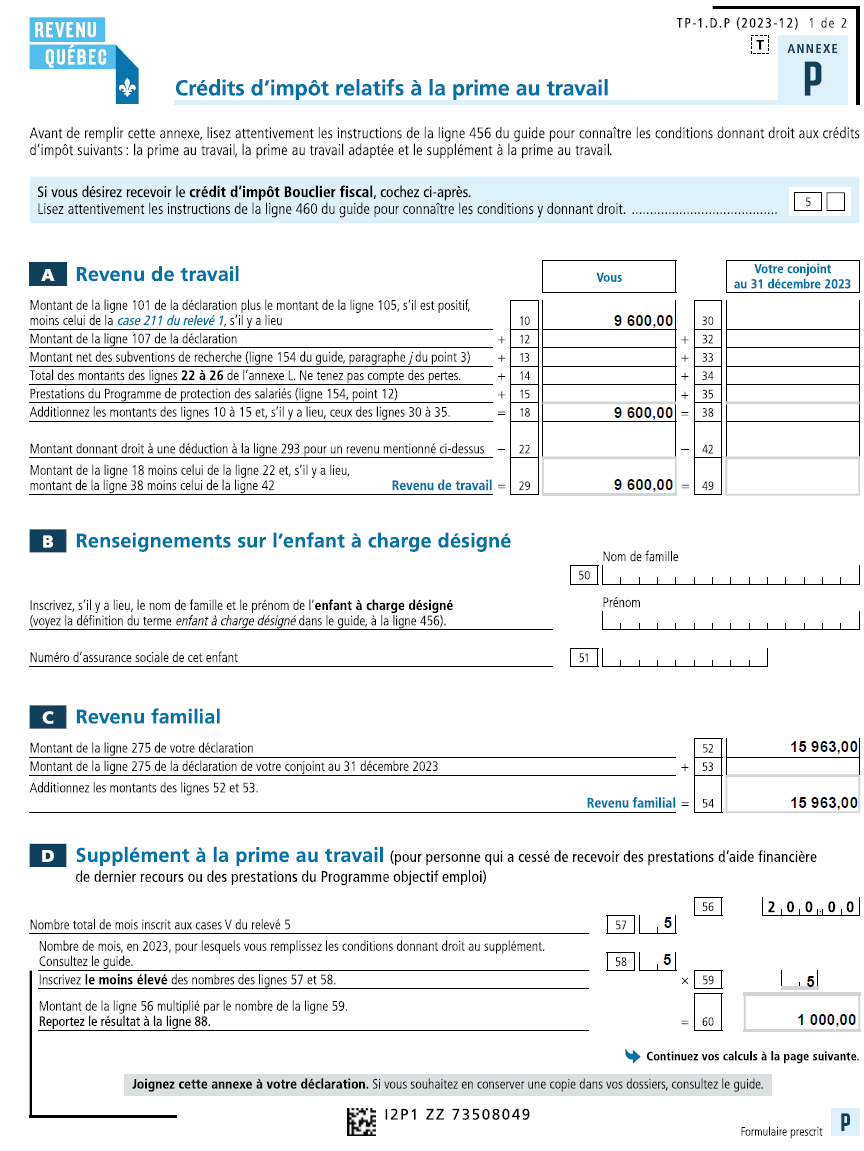
\includegraphics[width=.9\textwidth]{exercice/7-4/Q3/AnnexePp1.png}
	\caption[]{Exercice 4, annexe~P, page 1}
	\label{fig:chap7Exercice4AnnexePp1}
\end{figure}

Page 2: figure~\ref{fig:chap7Exercice4AnnexePp2}.
\begin{figure}
	\centering
	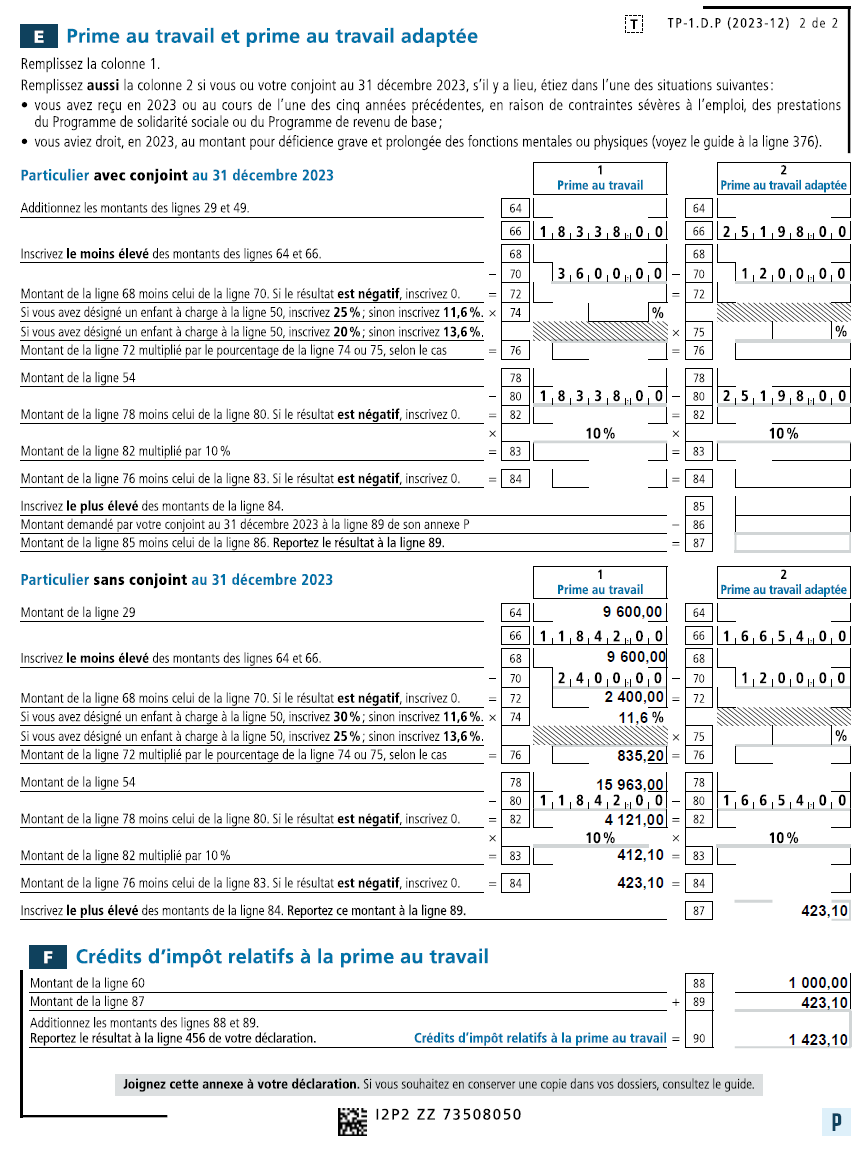
\includegraphics[width=.9\textwidth]{exercice/7-4/Q3/AnnexePp2.png}
	\caption[]{Exercice 4, annexe~P, page 2}
	\label{fig:chap7Exercice4AnnexePp2}
\end{figure}

\begin{question}
	Gaston et Nancy sont conjoints de fait. Ils ont un enfant né le 8~juillet~2018 (5~ans). En 2023, Gaston a eu un revenu d'emploi de \numprint{13700}~\$ et Nancy, de \numprint{15300}~\$. Le montant inscrit à la ligne~23600 (revenu net) de la déclaration T1 de Gaston est \numprint{13598}~\$ et celui de Nancy est de \numprint{15182}~\$.
	
	Nancy peut-elle demander l'Allocation canadienne pour les travailleurs? Si elle peut réclamer l'allocation, à combien a-t-elle droit? À quelle ligne de sa T1 Nancy devrait-elle réclamer ce montant? Remplissez l'\href{https://www.canada.ca/fr/agence-revenu/services/formulaires-publications/trousses-impot-toutes-annees-imposition/trousse-generale-impot-prestations/quebec/5005-s6.html}{annexe~6} de Nancy pour établir le montant que le couple pourrait réclamer, le cas échéant.
\end{question}
annexe~6, pages 2 à 4: figures~\ref{fig:chap7Exercice4Annexe6p2}, \ref{fig:chap7Exercice4Annexe6p3} et \ref{fig:chap7Exercice4Annexe6p4}. Nancy peut réclamer \numprint{3522,38}~\$ à la ligne~45300 de sa T1.

\begin{figure}
	\centering
	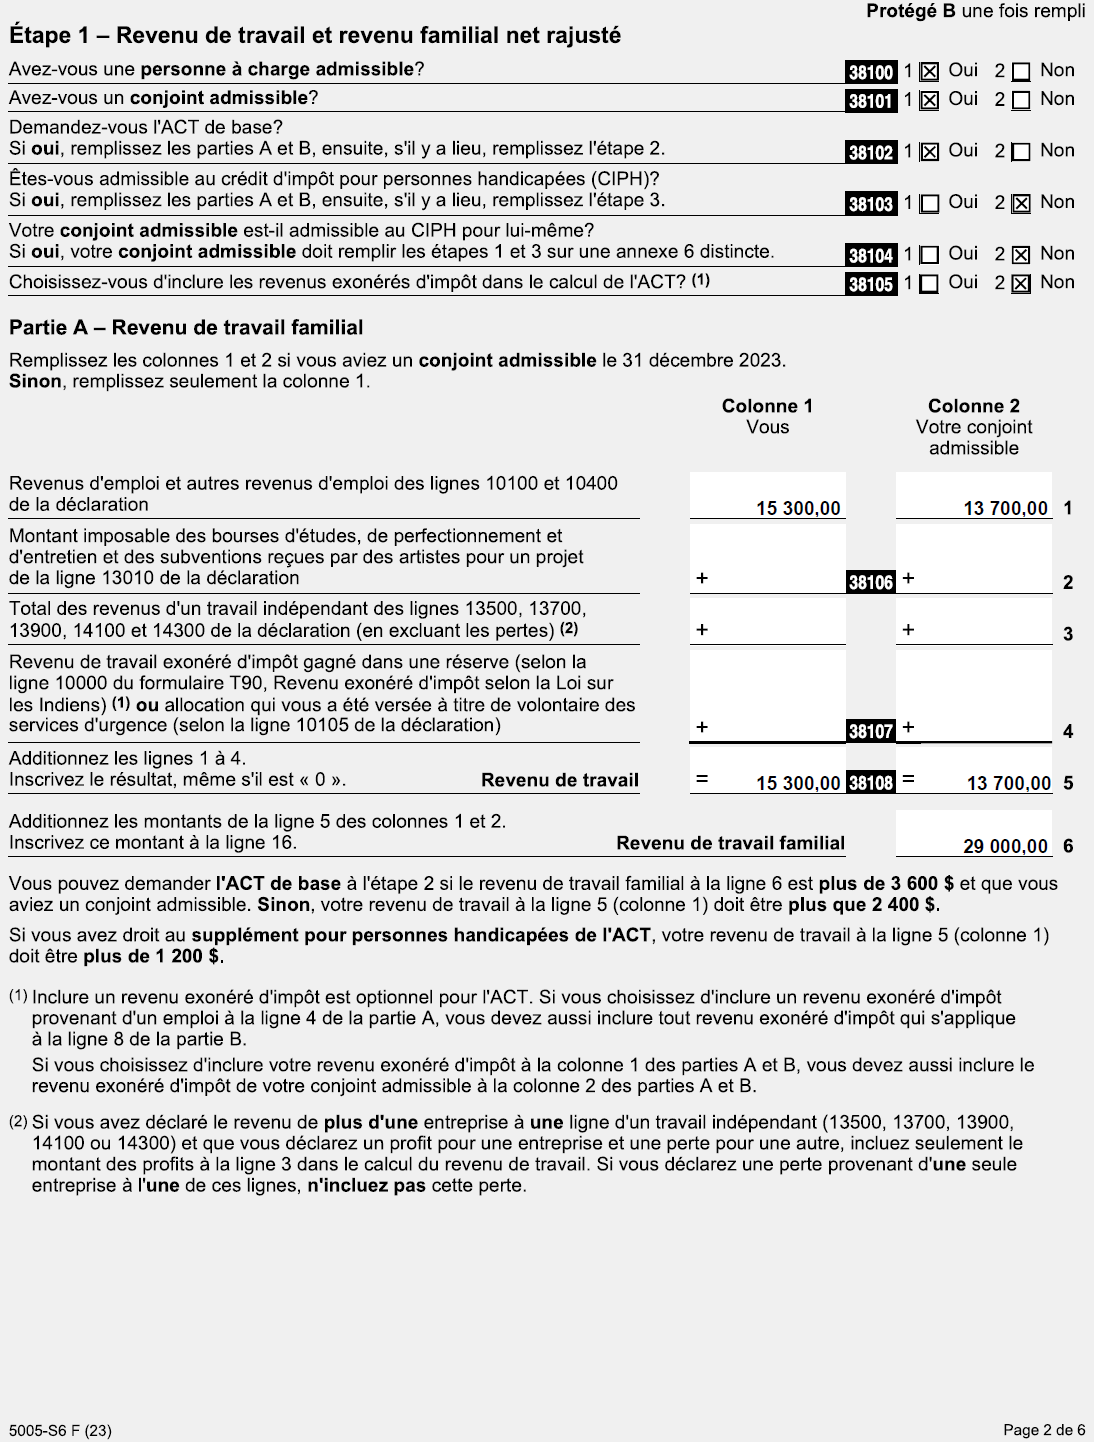
\includegraphics[width=.9\textwidth]{exercice/7-4/Q4/Annexe6p2.png}
	\caption[]{Exercice 4, annexe~6, page 2}
	\label{fig:chap7Exercice4Annexe6p2}
\end{figure}
\begin{figure}
	\centering
	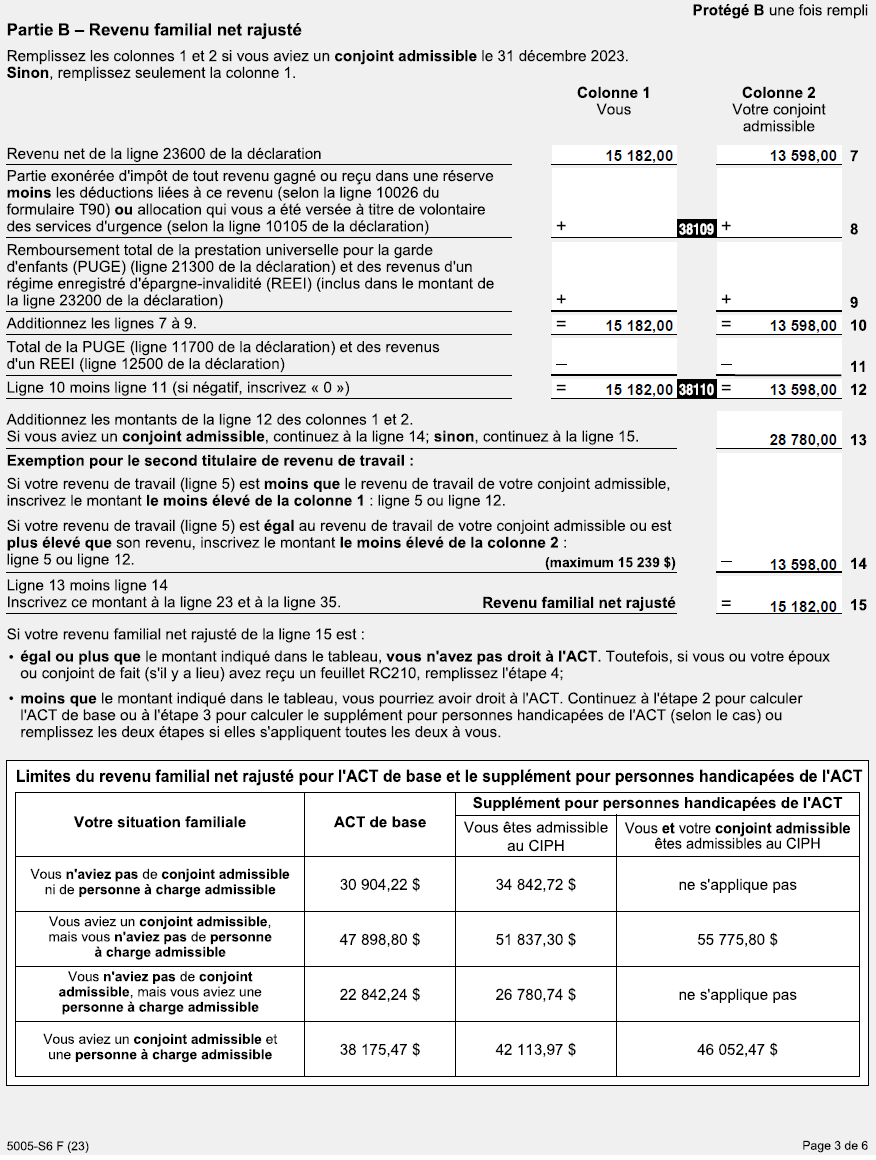
\includegraphics[width=.9\textwidth]{exercice/7-4/Q4/Annexe6p3.png}
	\caption[]{Exercice 4, annexe~6, page 3}
	\label{fig:chap7Exercice4Annexe6p3}
\end{figure}
\begin{figure}
	\centering
	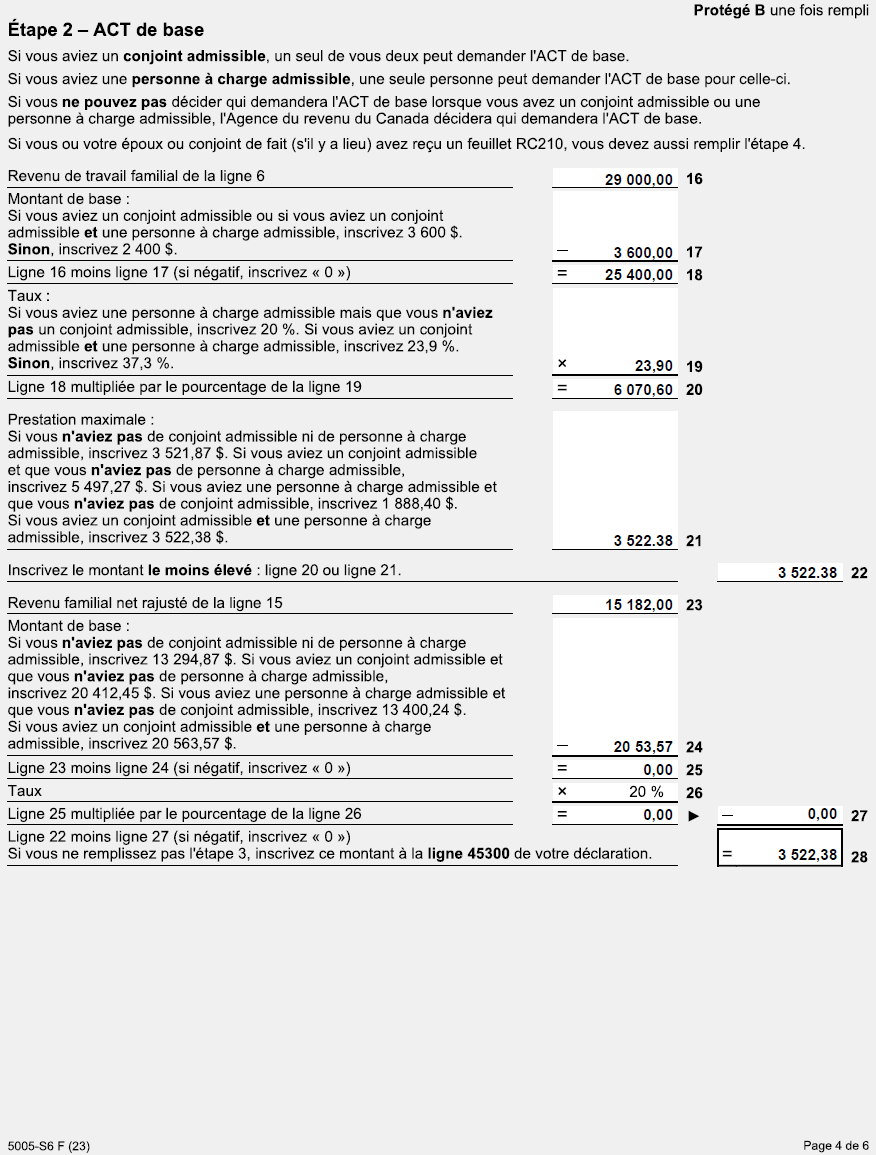
\includegraphics[width=.9\textwidth]{exercice/7-4/Q4/Annexe6p4.png}
	\caption[]{Exercice 4, annexe~6, page 4}
	\label{fig:chap7Exercice4Annexe6p4}
\end{figure}

\begin{question}
	Le 20~novembre~2022, Zihan Wang a signé un contrat avec un entrepreneur qualifié pour moderniser son système de traitement des eaux usées résidentiel. Elle a déjà réclamé \numprint{4500}~\$ en crédit d'impôt pour l'année d'imposition 2022. Elle a payé le montant final de \numprint{4000}~\$ dû en juin~2023.
	
	Quel montant peut-elle réclamer comme crédit d'impôt pour l'année d'imposition 2023?
\end{question}
Le montant du crédit qu'elle peut demander est de 20~\% du montant payé dans l'année d'imposition pourvu qu'elle ne dépasse pas le crédit cumulatif maximal de \numprint{5500}~\$.

Elle peut donc réclamer 20~\% de \numprint{4000}~\$, soit 800~\$, moins de \numprint{1000}~\$ (\numprint{5500}~\$ $-$ \numprint{4500}~\$) du crédit d'impôt disponible.



\section{Sommaire du chapitre}
\begin{itemize}[label=\twemoji{star}]
	\item Indemnités pour accident de travail
	\item Aide sociale et indemnités spécifiques au Québec
	\item Prestations du Régime de rentes du Québec, de l'assurance-emploi et du Régime québécois d'assurance parentale
	\item Remboursement de l'assurance-emploi et des prestations COVID
	\item Dons
	\item Crédit pour l'achat d'une habitation
	\item Aide financière accordée par les gouvernements aux contribuables et aux familles à faible revenu.
\end{itemize}
